\documentclass[
	12pt,				% tamanho da fonte
	openany,			% capítulos começam em pág ímpar (insere página vazia caso preciso)
	oneside, 			% oneside - twoside
	a4paper,			% tamanho do papel.
	chapter=TITLE,		% títulos de capítulos convertidos em letras maiúsculas
	section=TITLE,		% títulos de seções convertidos em letras maiúsculas
	sumario=tradicional,	
	%subsection=TITLE,	% títulos de subseções convertidos em letras maiúsculas
	%subsubsection=TITLE,% títulos de subsubseções convertidos em letras maiúsculas
	english,			% idioma adicional para hifenização
	brazil,				% o último idioma é o principal do documento
	]{abntex2}

% ---------------------------------------------------------------------------
% Inclui os comandos do projeto
% ---------------------------------------------------------------------------
% -----------------------------------------------------------------------------
% Pacotes fundamentais
% -----------------------------------------------------------------------------
\usepackage{xcolor}
\newcommand\myworries[1]{\textcolor{red}{[#1]}}
\usepackage{lmodern}		% Usa a fonte Latin Modern (Serifada, tipo Times New Roman
%\usepackage{helvet}		% Usa a fonte Helvetica (Tipo Arial)
%\renewcommand{\familydefault}{\sfdefault} tira o serifado
\usepackage[T1]{fontenc}		% Selecao de codigos de fonte.
\usepackage[utf8]{inputenc}		% Codificacao do documento (conversão automática dos acentos)
\usepackage{indentfirst}		% Indenta o primeiro parágrafo de cada seção.
\usepackage{color}				% Controle das cores
\usepackage{tikz}				% Inclusão de gráficos
\usepackage{graphicx}			% Inclusão de gráficos
\usepackage{microtype} 			% para melhorias de justificação
% -----------------------------------------------------------------------------
% Pacotes adicionais, usados no anexo do modelo de folha de identificação
% -----------------------------------------------------------------------------
\usepackage{multicol}
\usepackage{multirow}
% -----------------------------------------------------------------------------
% Pacotes adicionais, usados apenas no âmbito do Modelo Canônico do abnteX2
% -----------------------------------------------------------------------------
\usepackage{lipsum}				% para geração de dummy text
% -----------------------------------------------------------------------------
% Pacotes de citações
% -----------------------------------------------------------------------------
\usepackage[brazilian,hyperpageref]{backref}	 % Paginas com as citações na bibliografia
\usepackage[alf,abnt-etal-list=3,abnt-etal-cite=3, abnt-emphasize=bf]{abntex2cite}	% Citações padrão ABNT
\usepackage{pdflscape}
\usepackage{footnote}
\usepackage{pdfpages}
\usepackage{caption}

% -----------------------------------------------------------------------------
% Pacotes adicionados por @leolleocomp
% -----------------------------------------------------------------------------
\usepackage{booktabs}
\usepackage{adjustbox}
\usepackage{subcaption}
\usepackage[labelfont=bf]{caption}
\usepackage{gensymb}
\usepackage{amsmath}
\usepackage{array}
% \usepackage{float}
\usepackage{xcolor,colortbl}
\usepackage{longtable}
\usepackage{scalefnt}
\usepackage{listings}			% inserir codigo fonte
\usepackage{morewrites} % necessário pois estamos screvendo muitos arquivos

% -----------------------------------------------------------------------------
% Pacotes adicionados por @Gabrielr2508
% -----------------------------------------------------------------------------
\usepackage{hyperref}

\usepackage{tocloft}
% -- permite a adição de células especiais em tabelas
\newcommand{\specialcell}[2][c]{%
  \begin{tabular}[#1]{@{}c@{}}#2\end{tabular}}

\newcounter{equationset}
\newcommand{\equationset}[1]{% \equationset{<caption>}
  \refstepcounter{equationset}% Step counter
  \noindent\makebox[\linewidth]{Equação ~\theequationset: #1}
 }

%-------------------------------------------------------------------------------
% Adequação dos títulos dos capitulos, seções, subseções às normas da Univasf
% Added by @Gabrielr2508
%-------------------------------------------------------------------------------
\renewcommand{\ABNTEXchapterfont}{\fontseries{b}}
\renewcommand{\ABNTEXchapterfontsize}{\normalsize}

\renewcommand{\ABNTEXsectionfont}{\fontseries{m}}
\renewcommand{\ABNTEXsectionfontsize}{\normalsize}

\renewcommand{\ABNTEXsubsectionfont}{\fontseries{b}}
\renewcommand{\ABNTEXsubsectionfontsize}{\normalsize}

\renewcommand{\ABNTEXsubsubsectionfont}{\fontseries{m}}
\renewcommand{\ABNTEXsubsubsectionfontsize}{\normalsize}

%-------------------------------------------------------------------------------
% CONFIGURAÇÕES DE PACOTES
% Configurações do pacote backref
%-------------------------------------------------------------------------------
% Usado sem a opção hyperpageref de backref
\renewcommand{\backrefpagesname}{Citado na(s) página(s):~}
% Texto padrão antes do número das páginas
\renewcommand{\backref}{}
% Define os textos da citação
\renewcommand*{\backrefalt}[4]{
	\ifcase #1 %
		%Nenhuma citação no texto.%
	\or
		Citado na página #2.%
	\else
		Citado #1 vezes nas páginas #2.%
	\fi}%

%-------------------------------------------------------------------------------
% Configurações de aparência do PDF final
%-------------------------------------------------------------------------------
% alterando o aspecto da cor azul
\definecolor{blue}{RGB}{41,5,195}

% informações do PDF
\makeatletter
\hypersetup{
     	%pagebackref=true,
		pdftitle={\@title},
		pdfauthor={\@author},
    	pdfsubject={\imprimirpreambulo},
	    pdfcreator={LaTeX with abnTeX2},
		pdfkeywords={abnt}{latex}{abntex}{abntex2}{relatório técnico},
		colorlinks=true,			% false: boxed links; true: colored links
    	linkcolor=black,				% color of internal links
    	citecolor=black,				% color of links to bibliography
    	filecolor=black,			% color of file links
		urlcolor=black,
		bookmarksdepth=4
}
\makeatother
% ---

% ---
% Espaçamentos entre linhas e parágrafos
% ---

% O tamanho do parágrafo é dado por:
\setlength{\parindent}{1.3cm}

% Controle do espaçamento entre um parágrafo e outro:
\setlength{\parskip}{0.2cm}  % tente também \onelineskip

%-------------------------------------------------------------------------------
% compila o indice
%-------------------------------------------------------------------------------
\makeindex
% ---

%-------------------------------------------------------------------------------
% Comando para inserir imagens de forma simples
%-------------------------------------------------------------------------------
\newcommand{\imagem}[4]
{%			\imagem{x.x}{nomeimg}{titulo}{fonte}
	\begin{figure}[!htb]
		\caption{\label{img:#2}#3}
		\begin{center}
			\includegraphics[scale=#1]{img/#2}
		\end{center}
        \legend{\textbf{Fonte:} #4}
	\end{figure}
}%

%-------------------------------------------------------------------------------
% Creio que esses comandos sejam para desenhar algo, aguardando explicações de @leolleocomp
%-------------------------------------------------------------------------------
\newcommand{\xx} {$\bigotimes$}
\newcommand{\oo} {$\bigcirc$}

%-------------------------------------------------------------------------------
% Biblioteca para códigos-fonte
%-------------------------------------------------------------------------------
\usepackage[newfloat=true]{minted}

%-------------------------------------------------------------------------------
% Caixas batutas - by @leolleocomp
%-------------------------------------------------------------------------------
\usepackage[most]{tcolorbox}
\tcbuselibrary{breakable}

\tcbuselibrary{minted}
\tcbset{listing engine=minted}

\definecolor{bg}{rgb}{0.95,0.95,0.95}

\SetupFloatingEnvironment{listing}{name=Código, listname=Lista de códigos}

%-------------------------------------------------------------------------------
% configuração do contador dos códigos-fonte - by @leolleocomp
% assim como as figuras, começa em 1
\newcounter{sourcecode}
%-------------------------------------------------------------------------------
%-------------------------------------------------------------------------------
% @leolleocomp
% stackoverflow code
% peguei da resposta abaixo
% https://stackoverflow.com/questions/24086366/change-latex-minted-listings-numbering-to-include-current-section?answertab=votes#tab-top
%-------------------------------------------------------------------------------
\makeatletter
\renewcommand*{\thelisting}{\thesourcecode}
\makeatother

%-------------------------------------------------------------------------------
% Peçam explicações a @leolleo
% WHO DID THIS?
%-------------------------------------------------------------------------------
\newcommand{\Ididthis}{
%	\legend{\textbf{Fonte:} O autor (\the\year).}
\legend{\textbf{Fonte:} O autor}
}

\newcommand{\Otherguydidthis}[1]{
	\legend{\textbf{Fonte:} \citeonline{#1}.}
}

%-------------------------------------------------------------------------------
% Comando para inserir códigos - by @leolleocomp
%-------------------------------------------------------------------------------
\newcommand{\sourcecode}[4]{
\begin{listing}[h]
	\refstepcounter{sourcecode}
	\caption{#1}
	\label{cmd:#2}
	\inputminted[linenos, bgcolor=bg, tabsize=4,breaklines]{#3}{codes/#4}
	\Ididthis
\end{listing}
}


% -----------------------------------------------------------------------------
% Pacotes adicionados por @ruanmed
% -----------------------------------------------------------------------------
\usepackage[binary-units=true]{siunitx}


%-------------------------------------------------------------------------------
% Comando para inserir códigos - by @ruanmed
%-------------------------------------------------------------------------------
\usepackage{caption}

\newenvironment{code}{\captionsetup{type=listing}}{}
\SetupFloatingEnvironment{listing}{name=Código}

\newcommand{\sourcecodenolist}[4]{
	\begin{code}
	    \refstepcounter{sourcecode}
        \captionof{listing}{#1 }
        \label{code:#2}
        \inputminted[linenos, bgcolor=bg, tabsize=4,breaklines]{#3}{codes/#4}
        \Wedidthis
    \end{code}
}

\newcommand{\sourcecodeinline}[2]{
	\mintinline[linenos, bgcolor=bg, tabsize=4,breaklines]{#1}{#2}
}


% CONFIGURACAO DO SUMARIO
%-------------------------------------------------------------------------------
% Modifica o espaçamento no sumário
% Nao ha espacos, exceto para as entradas de capitulos
\setlength{\cftbeforeparagraphskip}{0pt}
\setlength{\cftbeforesubsectionskip}{0pt}
\setlength{\cftbeforesectionskip}{0pt}
\setlength{\cftbeforesubsubsectionskip}{0pt}
\setlength{\cftbeforechapterskip}{\onelineskip}

% Alteração da indentação dos itens do sumário
\cftsetindents{chapter}{0pt}{42pt}
\cftsetindents{section}{0pt}{42pt}
\cftsetindents{subsection}{0pt}{42pt}
\cftsetindents{subsubsection}{0pt}{42pt}

% Modifica a formatacao dos textos

% Secao Primaria (Chapter): Caixa alta, Negrito, tamanho 12
\makeatletter
\settocpreprocessor{chapter}{%
  \let\tempf@rtoc\f@rtoc%
  \def\f@rtoc{%
  \texorpdfstring{\bfseries\MakeTextUppercase{\tempf@rtoc}}{\tempf@rtoc}}%
}
\makeatother

% Novo list of (listings) para QUADROS
% retirado de https://github.com/abntex/abntex2/wiki/HowToCriarNovoAmbienteListing

\newcommand{\quadroname}{Quadro}
\newcommand{\listofquadrosname}{Lista de quadros}

\newfloat[chapter]{quadro}{loq}{\quadroname}
\newlistof{listofquadros}{loq}{\listofquadrosname}
\newlistentry{quadro}{loq}{0}

% configurações para atender às regras da ABNT
\setfloatadjustment{quadro}{\centering}
\counterwithout{quadro}{chapter}
\renewcommand{\cftquadroname}{\quadroname\space}
\renewcommand*{\cftquadroaftersnum}{\hfill--\hfill}

% Configuração de posicionamento padrão:
\setfloatlocations{quadro}{hbtp}


% ---------------------------------------------------------------------------
% IDENTIFICAÇÃO
% ---------------------------------------------------------------------------
\titulo{

SISTEMA EMBARCADO PARA AQUISIÇÃO DE DADOS E TELEMETRIA DE MINIFOGUETES
INTERMEDIÁRIO E AVANÇADO

}
\autor{JOSE ADOLFO DE CASTRO NETO}
\local{JUAZEIRO - BA}
\orientador{Prof. Dr. Max Santana Rolemberg Farias}
%\coorientador{M. Sc. Osvaldo Campelo de Mello Vasconselos}
\instituicao{
UNIVERSIDADE FEDERAL DO VALE DO SÃO FRANCISCO
	\par
CURSO DE GRADUAÇÃO EM ENGENHARIA DE COMPUTAÇÃO}
\tipotrabalho{Trabalho de Conclusão de Curso}
\preambulo{Trabalho apresentado à Universidade Federal do Vale do São Francisco - Univasf, Campus Juazeiro, como requisito da obtenção do título de Bacharel em Engenharia de Computação.}


% -----------------------------------------------------------------------------
% CONFIGURACAO DO SUMARIO - by @Gabrielr2508
% Precisa estar aqui, por isso não foi para o commands.tex, não descobrimos o motivo, %caso saiba, por favor, faça um pull request! :D
% -----------------------------------------------------------------------------
% Secao primaria (Chapter) Caixa alta, Negrito, tamanho 12
\makeatletter
\renewcommand*{\l@chapter}[2]{%
  \l@chapapp{\uppercase{#1}}{#2}{\cftchaptername}}
\makeatother
% Secao secundaria (Section) Caixa baixa, Negrito, tamanho 12
\renewcommand{\cftsectionfont}{\uppercase} %ponha \rmfamily se quiser serifadas...

% Secao terciaria (Subsection) Caixa baixa, negrito, tamanho 12
\renewcommand{\cftsubsectionfont}{\bfseries}

% Secao quaternaria (Subsubsection) Caixa baixa, tamanho 12
\renewcommand{\cftsubsubsectionfont}{\normalfont}

% Seção quinaria (subsubsubsection) Caixa baixa, sem negrito, tamanho 12
\renewcommand{\cftparagraphfont}{\normalfont\itshape}

% -----------------------------------------------------------------------------
% Início do TCC 
% -----------------------------------------------------------------------------
\begin{document}

	\frenchspacing % Retira espaço extra obsoleto entre as frases.
	
	\pretextual
		
%--------------------------------------------------------------------------------
% Constrói a capa com base na seção de identificação do main.tex
%--------------------------------------------------------------------------------
\begin{capa}
    \setlength{\belowcaptionskip}{0pt}
    \setlength{\abovecaptionskip}{0pt}
    \setlength{\intextsep}{-18pt}
        \begin{figure}[h]
    		\begin{center}
    		    
\includegraphics[scale=.5]{img/NEW_LOGO_UNIVASF.jpg}
    		\end{center}
    	\end{figure}

        %
\includegraphics[scale=0.6]{img/univasf.jpg}
        \center
    	{\ABNTEXchapterfont\large\imprimirinstituicao}

    	\vspace*{2cm}
    	    {\imprimirautor}
    	\vspace*{2cm}
        \begin{center}
    		\ABNTEXchapterfont\bfseries\large\imprimirtitulo
        \end{center}
    	\vfill

    	\ABNTEXchapterfont\bfseries\large\imprimirlocal\\
    	\the\year

    	\vspace*{1cm}
\end{capa}
%--------------------------------------------------------------------------------
% Constrói a folha de rosto com base na seção de identificação do main.tex
%--------------------------------------------------------------------------------
\begin{folhaderosto}
    \center
    	{\ABNTEXchapterfont\large\imprimirinstituicao}

		\vspace*{2cm}
    	    {\imprimirautor}
    	\vspace*{2cm}
		\vspace*{\fill}

		{\ABNTEXchapterfont\bfseries\large\imprimirtitulo}
		\vspace*{\fill}

		{\hspace{.45\textwidth}
		\begin{minipage}{.5\textwidth}
			\SingleSpacing
			\imprimirpreambulo \\ \\

			{\imprimirorientadorRotulo~\imprimirorientador\par}
			{\imprimircoorientadorRotulo~\imprimircoorientador\par}

		\end{minipage}%
		\vspace*{\fill}}%
		\vspace*{\fill}
			\ABNTEXchapterfont\bfseries\large\imprimirlocal\\
			\the\year
		\vspace*{1cm}
\end{folhaderosto}

%--------------------------------------------------------------------------------
% Constrói a ficha catalográfia com base na seção de identificação do main.tex
% Está comentado porque no final das contas a biblioteca do seu campus que gera a
% numeração, você pode adicionar os numeros aqui, ou anexar o pdf gerado por eles
% ao documento.
%--------------------------------------------------------------------------------
%\begin{fichacatalografica}
%	\vspace*{\fill}					% Posição vertical
%	\hrule							% Linha horizontal
%	\begin{center}					% Minipage Centralizado
%	\begin{minipage}[c]{12.5cm}		% Largura
%
%	\imprimirautor
%
%	\hspace{0.5cm} \imprimirtitulo  / \imprimirautor. --
%	\imprimirlocal, \the\year-
%
%	\hspace{0.5cm} xx p. : il. (algumas color.) ; 30 cm.\\
%
%	\hspace{0.5cm} \imprimirorientadorRotulo~\imprimirorientador\\
%
%	\hspace{0.5cm}
%	\parbox[t]{\textwidth}{\imprimirtipotrabalho~--~\imprimirinstituicao,
%	\the\year.}\\
%
%	\hspace{0.5cm}
%		1. Palavra-chave1.
%		2. Palavra-chave2.
%		I. Orientador.
%		II. Universidade xxx.
%		III. Faculdade de xxx.
%		IV. Título\\
%
%	\hspace{8.75cm} CDU 02:141:005.7\\
%
%	\end{minipage}
%	\end{center}
%	\hrule
%\end{fichacatalografica}

%--------------------------------------------------------------------------------
% Anexando a ficha catalogáfica e a folha de aprovação
%--------------------------------------------------------------------------------
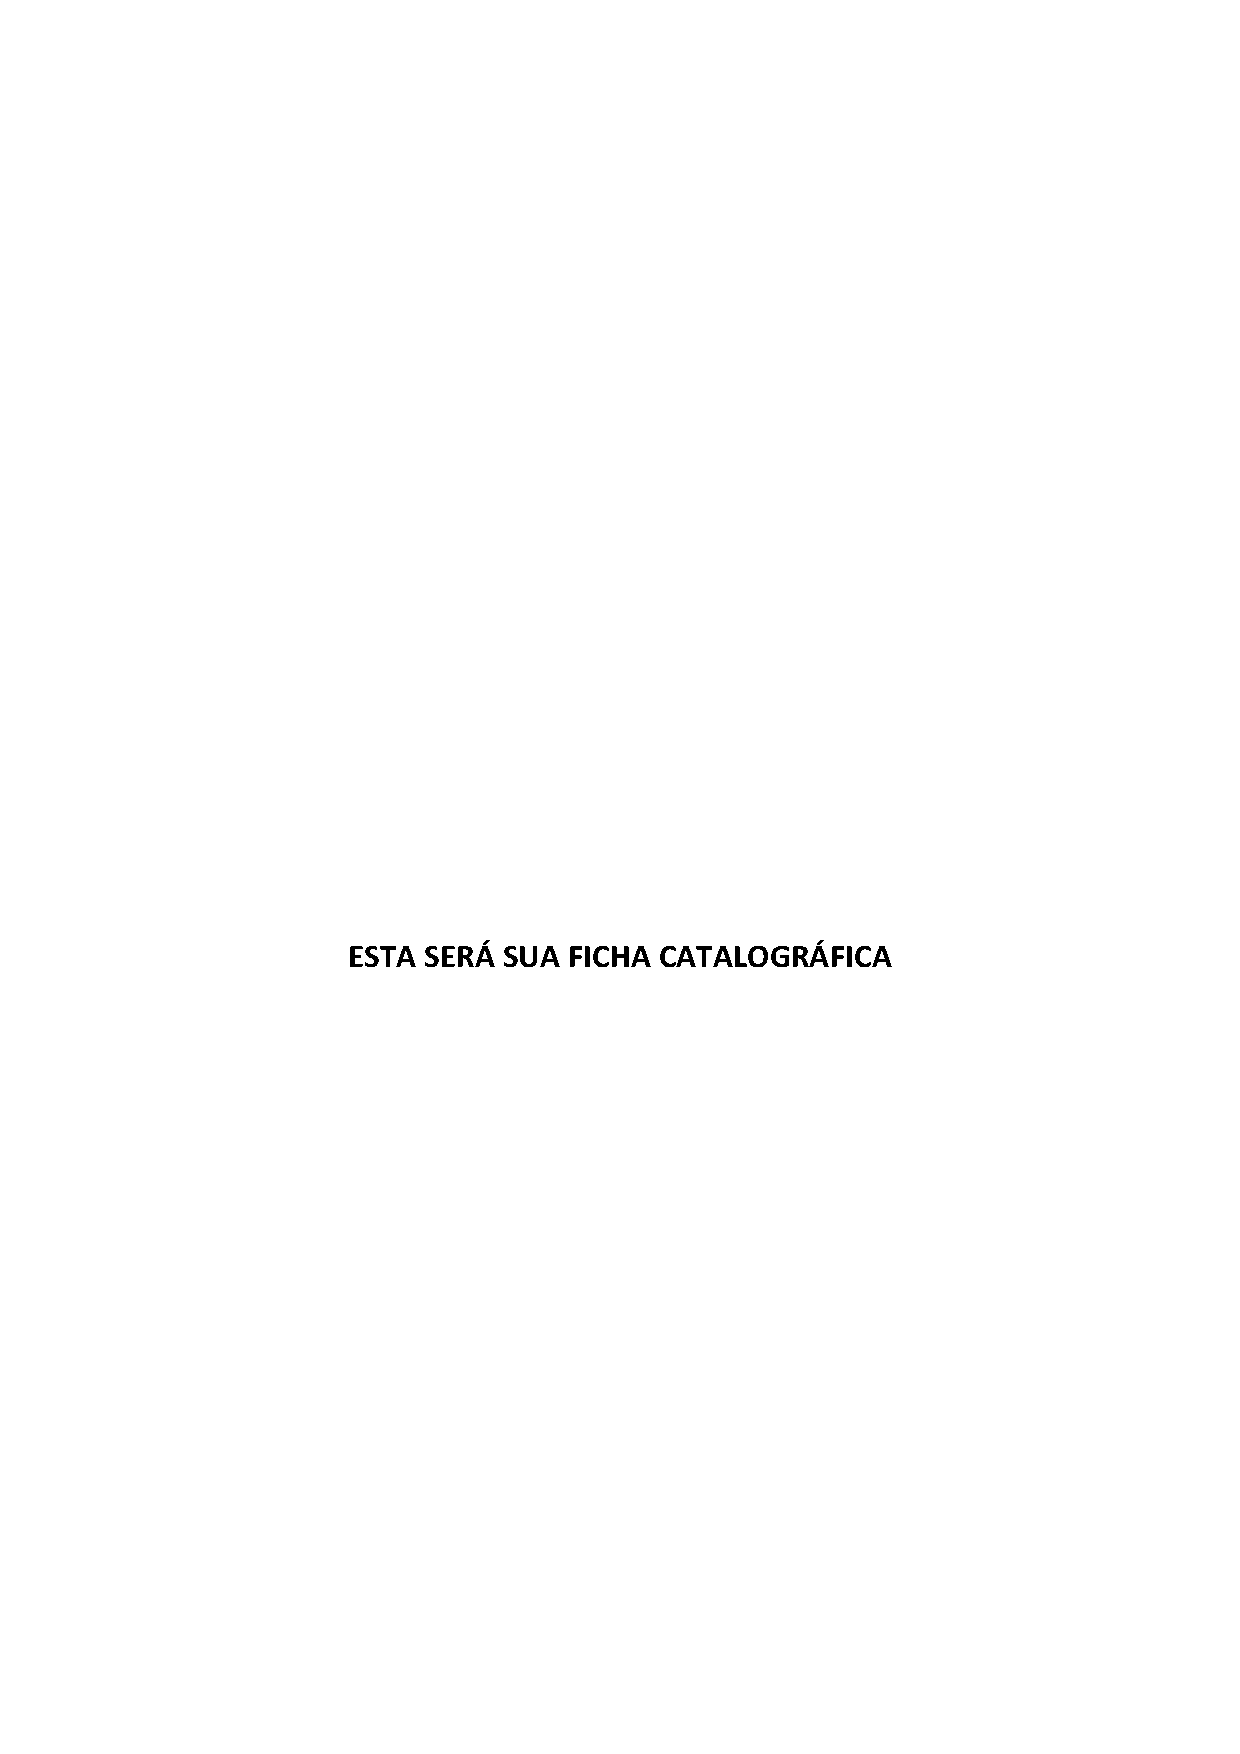
\includepdf[pages=-]{anexos/ficha.pdf}

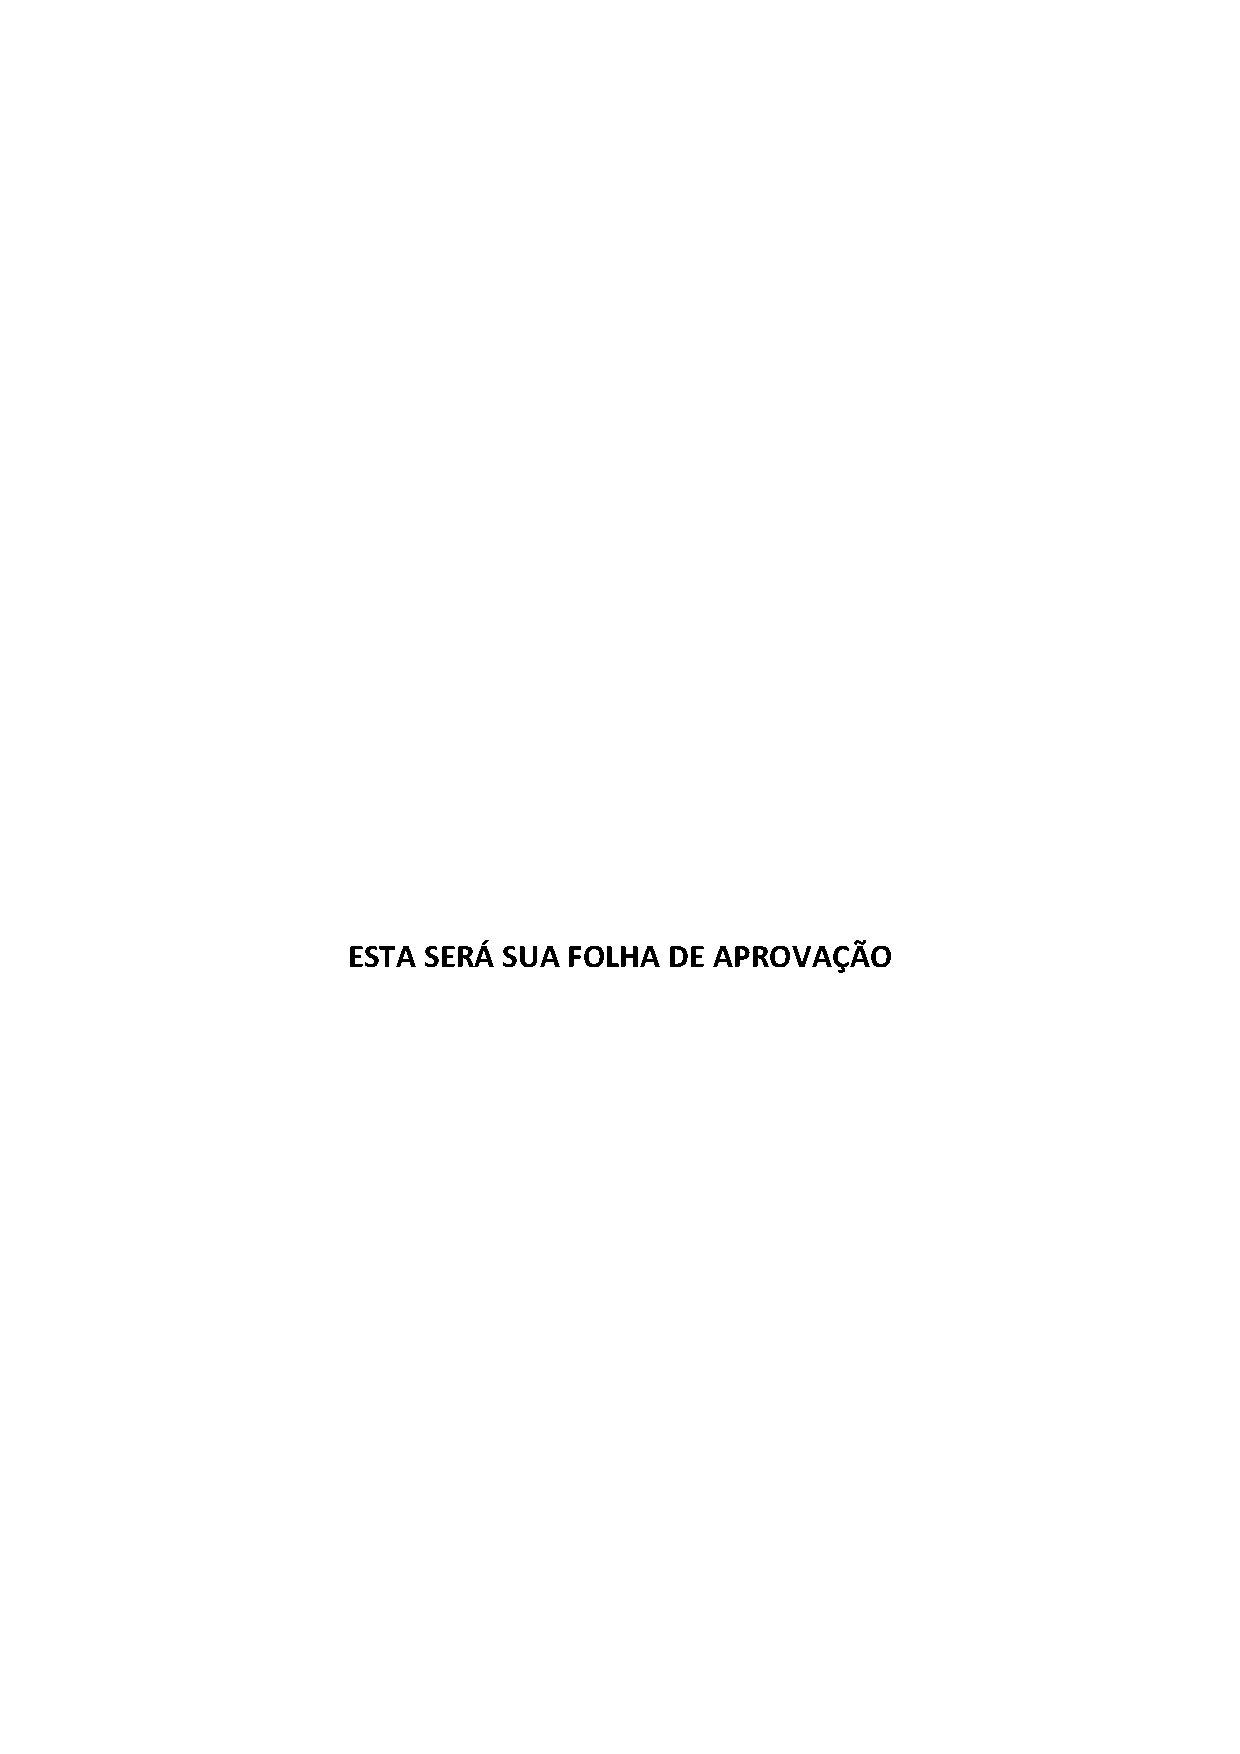
\includepdf[pages=-]{anexos/aprovacao.pdf}

%%--------------------------------------------------------------------------------
% Insere a folha de aprovação 
%--------------------------------------------------------------------------------
\begin{folhadeaprovacao}
	\begin{center}
		{\ABNTEXchapterfont\bfseries\large\imprimirinstituicao}
		\vspace*{\fill}

		{\ABNTEXchapterfont\bfseries\large FOLHA DE APROVAÇÃO}
		\vspace*{\fill}

		{\ABNTEXchapterfont\bfseries\large\imprimirautor}

		\vspace*{\fill}\vspace*{\fill}
		{\ABNTEXchapterfont\bfseries\large\imprimirtitulo}
		\vspace*{\fill}

		{\hspace{.45\textwidth}
		\begin{minipage}{.5\textwidth}
			\SingleSpacing
			\ABNTEXchapterfont\imprimirpreambulo \\ \\

			% {\ABNTEXchapterfont\imprimirorientadorRotulo~\imprimirorientador\par}
			% {\ABNTEXchapterfont\imprimircoorientadorRotulo~\imprimircoorientador\par}

		\end{minipage}%
		\vspace*{\fill}}
	\end{center}

	\vspace*{\fill}	
	
	\begin{center}
		% \ABNTEXchapterfont\large Aprovado em: \_\_\_\_ de \_\_\_\_\_\_\_\_ de 2020.
		\ABNTEXchapterfont\large Aprovado em: de de 2022.
	\end{center}

	\vspace*{\fill}
	
	\begin{center}
			 \ABNTEXchapterfont\bfseries\large Banca Examinadora
	\end{center}
		
	\ABNTEXchapterfont\assinatura{Rosalvo Ferreira de Oliveira Neto, Doutor, Universidade Federal do Vale do São Francisco}	
	\ABNTEXchapterfont\assinatura{Juracy Emanuel Magalhães da Franca, Mestre, Universidade Federal do Vale do São Francisco}
	\ABNTEXchapterfont\assinatura{Marcus Vinícius Midena Ramos, Doutor, Universidade Federal do Vale do São Francisco}
	\vspace*{\fill}

	 
\end{folhadeaprovacao}

\setlength{\ABNTEXsignwidth}{12cm}

%--------------------------------------------------------------------------------
% Está comentado pelo mesmo motivo da ficha catalográfica
%--------------------------------------------------------------------------------
%\begin{folhadeaprovacao}
%	\begin{center}
%	    {\ABNTEXchapterfont\bfseries\large\imprimirinstituicao}
%	    \vspace*{\fill}
%
%	    {\ABNTEXchapterfont\bfseries\large FOLHA DE APROVAÇÃO}
%	    \vspace*{\fill}
%
%	    {\ABNTEXchapterfont\bfseries\large\imprimirautor}
%
%	    \vspace*{\fill}\vspace*{\fill}
%	    {\ABNTEXchapterfont\bfseries\large\imprimirtitulo}
%	    \vspace*{\fill}
%
%	    {\hspace{.45\textwidth}
%		\begin{minipage}{.5\textwidth}
%			\SingleSpacing
%			\ABNTEXchapterfont\imprimirpreambulo \\ \\
%
%			{\ABNTEXchapterfont\imprimirorientadorRotulo~\imprimirorientador\par}
%			{\ABNTEXchapterfont\imprimircoorientadorRotulo~\imprimircoorientador\par}
%
%		\end{minipage}%
%	    \vspace*{\fill}}
%	\end{center}
%
%	\vspace*{\fill}
%
%	\begin{center}
%			 \ABNTEXchapterfont\large Aprovado em: \_\_\_\_ de \_\_\_\_ de 2017
%	\end{center}

%	\vspace*{\fill}

%	\begin{center}
%			 \ABNTEXchapterfont\bfseries\large Banca Examinadora
%	\end{center}
%
%   \ABNTEXchapterfont\assinatura{Fábio Nelson de Sousa Pereira, Mestre, Universidade Federal do Vale do São Francisco}
%	\ABNTEXchapterfont\assinatura{Jorge Luis Cavalcanti Ramos, Doutor, Universidade Federal do vale do São Francisco}
%  \ABNTEXchapterfont\assinatura{Ricardo Argenton Ramos, Doutor, Universidade Federal do Vale do São Francisco}
%	 \vspace*{\fill}


%\end{folhadeaprovacao}

%--------------------------------------------------------------------------------
% Insere a epígrafe
%--------------------------------------------------------------------------------
\newpage
\vspace*{\fill}
\begin{flushright}
		
\end{flushright}

%--------------------------------------------------------------------------------
% Seção de agradecimentos
%--------------------------------------------------------------------------------
\begin{agradecimentos}
Eu agradeço primeiramente a Deus, por ter me permitido chegar até aqui com alegria e saúde. Aos meus pais Edeilton e Iolanda que me apoiaram durante tanto tempo. Agradeço  aos meus colegas da universidade, no qual tive várias conversas interessantes ao longo da minha graduação. Agradeço aos professores das mais diversas disciplinas, tanto do colegiado de Engenharia da computação como também do colegiado de engenharia elétrica, pelo conhecimento compartilhado e ajuda oferecida, que me fez abrir os olhos e aumentar ainda mais a minha curiosidade sobre as diversas áreas do  conhecimento. Agradeço ao meu orientador Max Santana, que aceitou me ajudar nesse trabalho de conclusão de curso, a Ruan de Medeiros e Ricado Argenton, por aceitarem ser avaliadores da banca de defesa. 
%lipsum[2-4]

\end{agradecimentos}

%--------------------------------------------------------------------------------
% Insere a segunda epígrafe
%--------------------------------------------------------------------------------
\begin{epigrafe}
    \vspace*{\fill}
	\begin{flushright}
		Se pude enxergar a tão grande distância, foi subindo nos ombros de gigantes.\\
		 \vspace{\baselineskip}
		\textbf{Isaac Newton}\\
		\textbf{Carta à Robert Hooke, 1676}
	\end{flushright}
\end{epigrafe}



%--------------------------------------------------------------------------------
% Seção de resumos
%--------------------------------------------------------------------------------
% resumo em português
\setlength{\absparsep}{18pt} % ajusta o espaçamento dos parágrafos do resumo
\begin{resumo}


Uma das fases mais importantes no desenvolvimento de minifoguetes depois da simulação é o teste prático. Esta fase validará de fato o desempenho que foi simulado, mas para isso é necessário ter um sistema embarcado dentro do minifoguete capaz de capturar as principais variáveis, armazená-las e transmiti-las para um computador em solo. A fim de contribuir com a equipe de foguetemodelismo chamada Cactus Rocket Design da Universidade Federal do Vale do São Francisco, este trabalho tem como objetivo a construção de dois sistemas. O primeiro sistema embarcado será responsável pela captura, armazenamento e envio por telemetria dos principais dados sobre o minifoguete. Já o segundo sistema será responsável por receber os dados e transmitir para um computador, para que possa ser armazenado em um arquivo txt, para futuros relatórios. Assim, evita-se a perda dos dados gravados no cartão micro SD caso ocorra à perda do foguete.









 \textbf{Palavras-chave}: \textit{Minifoguete, Sistema Embarcado, Cactus Rocket Design, Telemetria}.

\end{resumo}

%---------------------------------------------------------------------------------
% resumo em inglês
\begin{resumo}[Abstract]
\begin{otherlanguage*}{english}



One of the most important phases in the development of mini-rockets after the simulation is the practical test. This phase will in fact validate the performance that was simulated, but for that it is necessary to have an embedded system inside the mini-rocket capable of capturing the main variables, storing them and transmitting them to a computer on the ground. In order to contribute to the model rocket team called Cactus Rocket Design at the Universidade Federal do Vale do São Francisco, this work aims to build two systems. The first embedded system will be responsible for capturing, storing and telemetry sending the main data about the mini-rocket. The second system will be responsible for receiving the data and transmitting it to a computer, so that it can be stored in a txt file for future reports. Thus, the loss of data recorded on the micro SD card is avoided if the rocket is lost. 







	\vspace{\onelineskip}

	\noindent
	\textbf{Key-words}: \textit{mini-rocket, Embedded System, Cactus Rocket Design, Telemetry  }.

\end{otherlanguage*}
\end{resumo}


%---------------------------------------------------------------------------------
% Insere lista de ilustrações
%---------------------------------------------------------------------------------
\begin{KeepFromToc} % Este comando evita que todas as seções dentro dele de apareçam no sumário
\pdfbookmark[0]{\listfigurename}{lof}
\listoffigures
%\addcontentsline{toc}{chapter}{Lista de Figuras}
\cleardoublepage


%---------------------------------------------------------------------------------
% Insere lista de tabelas
%---------------------------------------------------------------------------------
\pdfbookmark[0]{\listtablename}{lot}
\listoftables
\cleardoublepage

%---------------------------------------------------------------------------------
% Insere lista de quadros
%---------------------------------------------------------------------------------
%\pdfbookmark[0]{\listofquadrosname}{loq}
%\listofquadros*
%\cleardoublepage

%---------------------------------------------------------------------------------
% Ajusta lista de código - alterar de figures para códigos - by @Gabrielr2508
%---------------------------------------------------------------------------------
\makeatletter
\let\l@listing\l@figure
\def\newfloat@listoflisting@hook{\let\figurename\listingname}
\makeatother

%---------------------------------------------------------------------------------
% Insere lista de códigos - by @leolleocomp
%---------------------------------------------------------------------------------
%\listoflistings

\end{KeepFromToc}

%---------------------------------------------------------------------------------
% Insere lista de abreviaturas e siglas
%---------------------------------------------------------------------------------







\begin{siglas}




%###    a    ###
%###    b    ###
\item[BAR] Brazilian Association of Rocketry (Associação Brasileira de Minifoguetes)
%###    c    ###
\item[CI] Circuito Integrado
\item[CTA] Centro Técnico Aeroespacial 
%###    d    ###
\item[DCTA] Departamento de Ciência e Tecnologia Aeroespacial 
\item[DOP] Dilution of precision (Diluição da precisão, ou diluição geométrica da precisão)
%###    e    ###
%###    f    ###
\item[FM] Foguetemodelo 
%###    g    ###
\item[GPS] Sistema de Posicionamento Global 
%###    h    ###
%###    i    ###
\item[ITA]  Instituto Tecnológico de Aeronáutica
%###    j    ###
%###    k    ###
%###    l    ###
%###    m    ###
\item[MFE] Minifoguete experimental 
%###    n    ###
%###    o    ###
%###    p    ###
\item[PCB] Printed Circuit Board (Placa de Circuito Impresso)
%###    q    ###
%###    r    ###
%###    s    ###
\item[SNR] Signal to Noise Ratio (Razão sinal ruído) 
%###    t    ###
%###    u    ###
%###    v    ###
\item[VLM-1] Veículo lançador de microssatélites
\item[VPP] Peak-to-peak voltage (tensão de pico a pico)
\item[VLS] Veículo lançador de satélites
%###    w    ###
%###    x    ###
%###    y    ###
%###    z    ###



\end{siglas}




%\begin{siglas}
%	\item[LI]       Lorem Ipsum
%    \item[LII]		Lorem Ipsum Ipsum

%\end{siglas}

%---------------------------------------------------------------------------------
% Insere o sumario
%---------------------------------------------------------------------------------
\pdfbookmark[0]{\contentsname}{toc}
\tableofcontents*
\cleardoublepage




	\textual
		\pagestyle{simple}
		%--------------------------------------------------------------------------------------
% Este arquivo contém a introdução, objetivos e organização do trabalho
%--------------------------------------------------------------------------------------

\chapter{Introdução}

%--------------------------------------------------------------------------------------



A admiração e a curiosidade da humanidade pelo espaço vêm desde a pré-história, mas apenas através das descobertas de Isaac Newton, no Cálculo e na Física há 300 anos, a humanidade pôde trilhar um caminho, ao menos teórico rumo ao espaço. Porém, as tecnologias básicas à exploração espacial como rádio, só foram inventadas já no final do século XIX, dois séculos depois das descobertas de Newton \cite{Burgess2021}. No início do Século XX, o físico experimental Robert Goddard ansiava por provar que os foguetes poderiam ser motores no vácuo através da 3° lei de Newton (ação e reação). Conseguindo construir e lançar o primeiro foguete de propulsão líquida em 1926 visto na figura\ref{fig:Primeiro-foguete}.









\begin{figure}[ht]
    \centering
    \caption{Dr. Robert H. Goddard é mostrado em pé com o primeiro foguete de propulsão líquida do mundo em Auburn, MA, 16 de março de 1926.}
    \begin{center}
        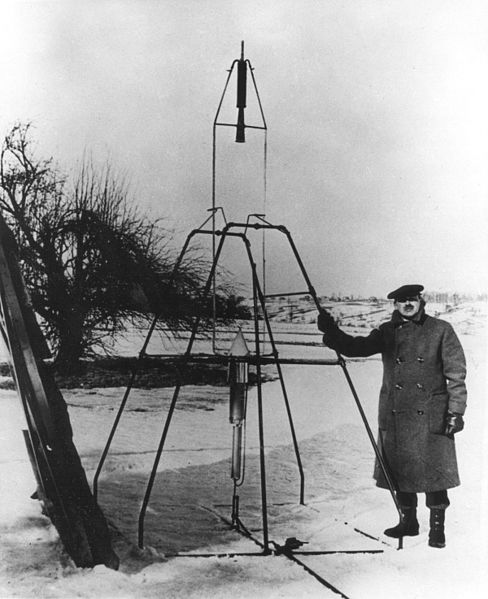
\includegraphics[width=0.35\textwidth]{img/primeirofoguete.jpg}
    \end{center}
    \vspace{-0.5cm}
    \legend{\ABNTEXfontereduzida \textbf{Fonte:} 
    \citeonline{Imagem_Primeiro_foguete}.}
   \label{fig:Primeiro-foguete}
\end{figure}.


Com o mundo entrando na Segunda Guerra Mundial, lamentavelmente a primeira aplicação dos foguetes não foi para o benefício da humanidade, sendo utilizado como meio de lançar bombas muito mais rápidas, sem os custos operacionais ou possíveis perdas de aviões e pilotos. Felizmente essa tecnologia só foi utilizada já no final da guerra, não causando tantos estragos. O míssil V2 mostrado na figura \ref{fig:foguete-V2} foi desenvolvido pelo engenheiro mecânico alemão Wernher Von Braun, Arthur Rudolph, Kurt H. Debus e outros. Logo depois da guerra, o míssil V2 foi utilizado para outras finalidades, por exemplo, responsável por tirar a 1° foto da terra a uma altitude acima da linha de Kármán \footnotemark{}  aproximadamente 104 km, em 1946.   


 




\begin{figure}[ht]
    \centering
    \caption{Míssil balístico V2 sendo preparado para lançamento em Cuxhaven, na Alemanha, 15 de  outubro de 1945.}
    \begin{center}
        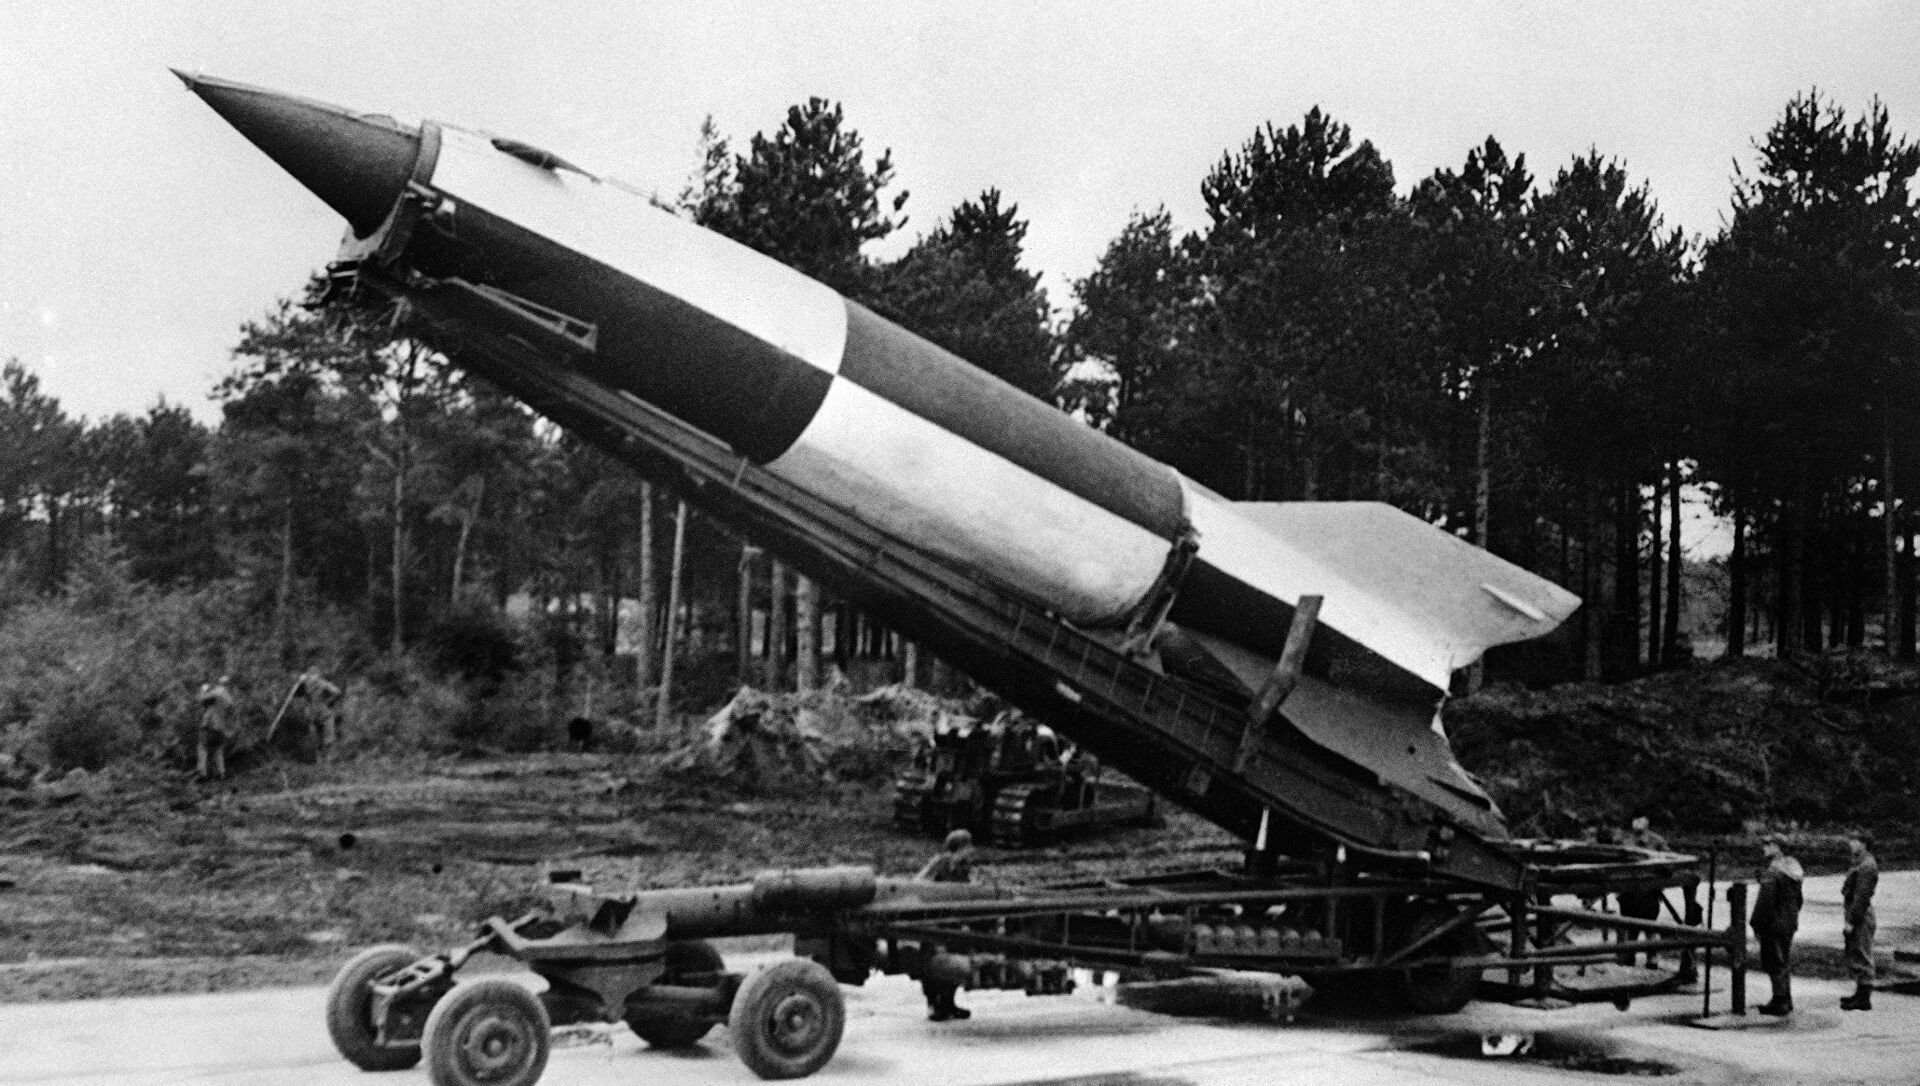
\includegraphics[width=0.5\textwidth]{img/missil_balistico_V2.jpg}
    \end{center}
    \vspace{-0.5cm}
    \legend{\ABNTEXfontereduzida \textbf{Fonte:} 
    \citeonline{Imagem_MissilV2}.}
    \label{fig:foguete-V2}
\end{figure}




.


Com o fim da Guerra, Países como os Estados Unidos (EUA) e a União Soviética (URSS) tiveram grande interesse nos cientistas e no projeto do V2, já que se tratava de uma tecnologia estratégica para o país. Tendo avanços significativos em ambos os lados como, no lado da URSS, o lançamento do primeiro satélite artificial da Terra, o Sputnik 1 em 1957, o primeiro homem e mulher a ficar na órbita da terra em 1961 e 1963, respectivamente. E pelo lado dos EUA, a chegada do homem à Lua, em 1969, através do foguete Saturno V como mostra a figura \ref{fig:Saturno-V}    \cite{UmaBreveHistoriadaConquistaEspacial}.
 

\begin{figure}[ht]
    \centering
    \caption{O foguete Saturno V preparado para o lançamento da missão Apollo 8 do Centro Espacial Kennedy em 1968.}
    \begin{center}
        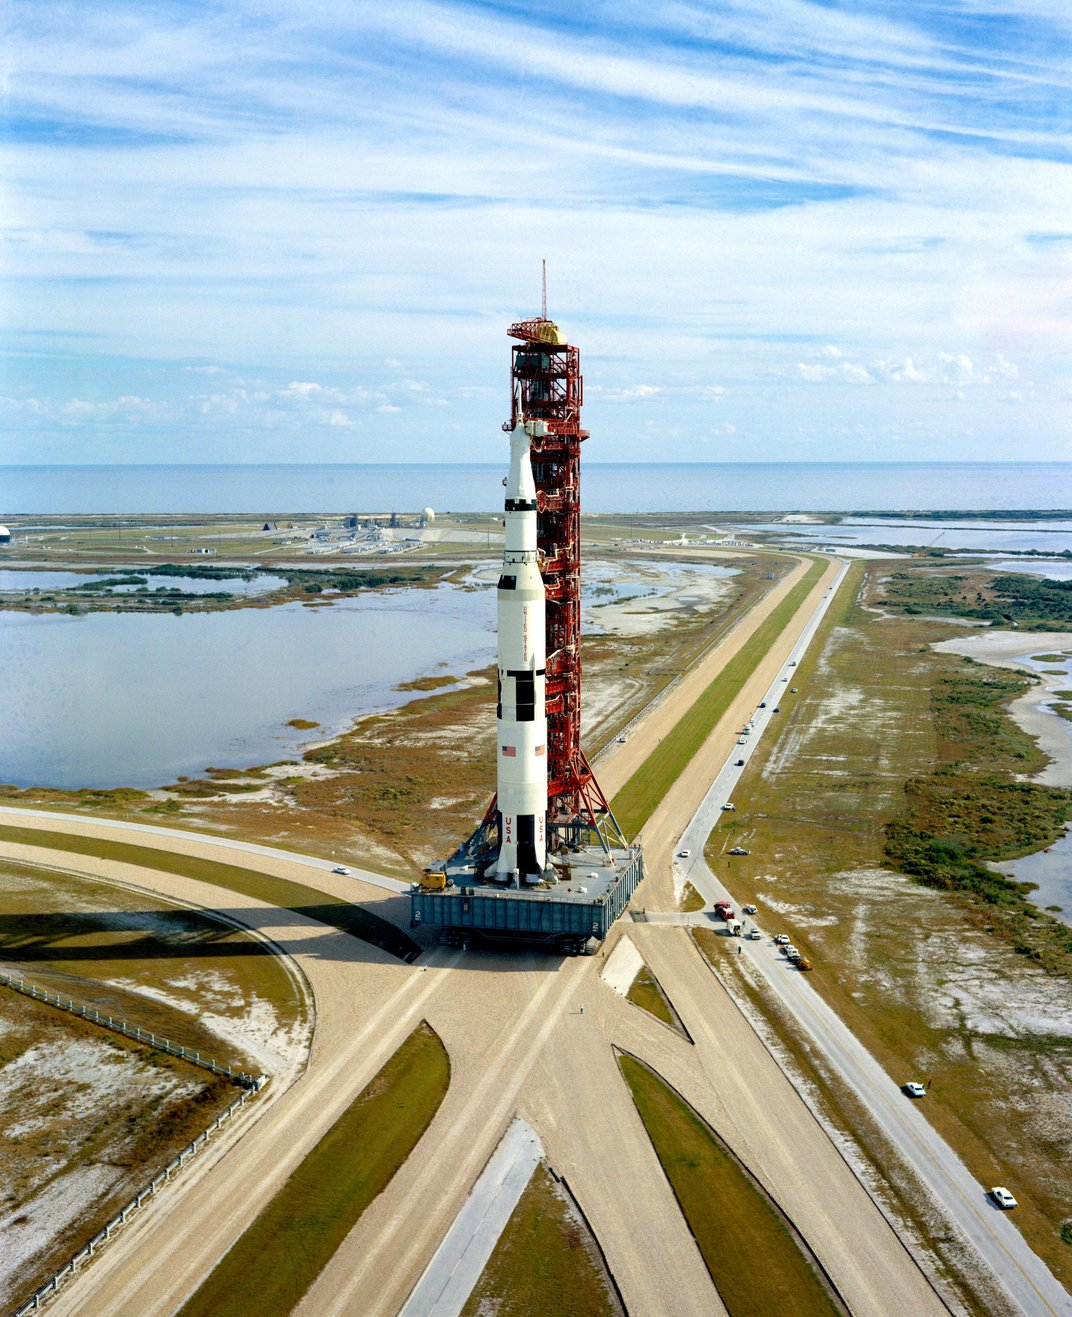
\includegraphics[width=0.35\textwidth]{img/saturn V.jpg}
    \end{center}
    \vspace{-0.5cm}
    \legend{\ABNTEXfontereduzida \textbf{Fonte:}
    \citeonline{Imagem_SaturnV}.}
    \label{fig:Saturno-V}
\end{figure}
.
 

\footnotetext{Linha de Kármán é utilizado para definir o limite entre a atmosfera terrestre e o espaço exterior que fica a uma altitude de 100 km acima do nível do mar.}





Já no Brasil, o Departamento de Ciência e Tecnologia Aeroespacial (DCTA) foi fundado em 1946, depois os principais institutos como o Centro Técnico Aeroespacial (CTA) e o Instituto Tecnológico de Aeronáutica (ITA) em 1950. Esses centros e institutos foram criados visando obter a autossuficiência do Brasil na formação de profissionais qualificados para trabalhar na área da aeronáutica e aeroespacial. Porém, só na década de 1960, o Brasil deu início ao desenvolvimento dos primeiros foguetes. Como os de sondagem que tem o propósito de levar pequenas cargas úteis para a alta atmosfera, realizando pesquisas e experiências \cite{INTRODUCAO_TECNOLOGIA_FOGUETES}.


O primeiro foi o Sonda I feito em 1967, o segundo o Sonda II em 1970 chegando a um apogeu  \footnotemark{} de 96 km, depois o  sonda III em 1976, com apogeu de 700 km. Até que em 1984 o auge da família com o sonda IV chegando a um apogeu de 700 km e conseguindo carregar até 500 kg de carga útil foi a base para a construção do Veículo lançador de satélites (VLS) \cite{Foguetes-AEB}.


Devido ao baixíssimo orçamento pelo governo e as grandes dificuldades na importação de componentes estratégicos devido aos embargos dos EUA, o programa do VLS só conseguiu realizar 3 tentativas com a última ocasionando a destruição da base e na morte de 21 pessoas em 2003. Ressurgindo apenas em 2010 o interesse em lançamentos de micro e nanossatélites e apenas em 2014 o Brasil em parceria com a Alemanha, deu início ao desenvolvendo do veículo de sondagem VS 50 que será base para a construção do veículo lançador de microssatélites (VLM-1). Com o novo projeto do VLM-1 o antigo VLS teve seu cancelamento definitivo em 2016 \cite{INTRODUCAO_TECNOLOGIA_FOGUETES}.



Visando possibilitar que estudantes possam participar de atividades voltadas ao desenvolvimento aeroespacial, a COBRUF Association é uma iniciativa privada New Space criada em 2012 por 10 estudantes de graduação da UFABC e que tem uma forte influência na coordenação de diversas operações experimentais de lançamento de foguetes com a Força Aérea Brasileira. Além disso, ela é responsável por promover diversas competições de foguetemodelismo nacional e internacional, impulsionando assim, o conhecimento técnico de diversos estudantes brasileiros nessa área tão escassa de profissionais\cite{Cobruf}.


Com o intuito de que a Universidade Federal do Vale do São Francisco -(UNIVASF) também entrasse nessa competição de foguetemodelismo, a equipe Cactus Rockets Design foi criada em 2019, por estudantes e professores. Visando contribuir com a equipe para que ela consiga alcançar o seu objetivo de construir foguetes modelos intermediários e avançados, esse trabalho de conclusão de curso foi desenvolvido para ajudar na coleta de dados dos sensores e na telemetria dos foguetes modelos projetados pela Cactus Rockets.



 \footnotetext{Apogeu na engenharia aeroespacial é a altura máxima em que o foguete pode atingir em relação a terra depois que todo o seu combustível é queimado.}

\newpage

\section{Justificativa}

A competição de foguetes organizada pela COBRUF dá a possibilidade para que estudantes de engenharia possam entrar em contato com o ambiente da engenharia aeroespacial, onde as necessidades e as exigências aos sistemas embarcados estão cada vez mais altas. Com o intuito de contribuir com a equipe Cactus Rockts em seu objetivo de construir foguetes intermediários e avançados, propomos um sistema embarcado para o foguete e um sistema externo no solo para receber os dados via telemetria. Através do sistema será possível obter os dados necessários para validar os cálculos e simulações feitas pela equipe e assim facilitar a identificação de erros de projeto e consequentemente favorecer melhorias futuras no desempenho dos foguetes projetados pela equipe Cactus Rockts.


\section{Objetivos gerais}

Possibilitar que a equipe de foguetemodelismo chamada Cactus Rockets Design da Universidade Federal do Vale do São Francisco possa obter os dados relevantes sobre os foguetes projetados. E assim, ser capaz de verificar se seus cálculos e simulações estão de acordo com a realidade mensurada de seus protótipos.



\section{Objetivos específicos}


\begin{itemize}
	\item Definir quais parâmetros são necessários e os sensores para mensurar tais parâmetros;
	
    \item Definir qual o microcontrolador será utilizado com base em um custo-benefício;
    
    \item Definir qual rádio apresenta um melhor custo-benefício para o projeto;
    
    \item Teste em bancada dos sensores;
    
    \item Teste em bancada do rádio;
    
    \item Teste do rádio em campo aberto para obter uma estimativa do alcance;
    
    \item Desenvolver o protótipo.
\end{itemize}





\section{Organização do trabalho}


O presente trabalho foi dividido em 3 etapas. A primeira etapa, trata-se de um resumo da história do foguete no mundo e no Brasil e a motivação para o desenvolvimento deste projeto. Na segunda, etapa é desenvolvida a fundamentação teórica que servirá como base para a realização deste trabalho. Por fim, a terceira etapa relata a metodologia utilizada neste projeto. Tendo no final da terceira etapa, um cronograma de atividades a serem executadas no Trabalho de conclusão II (TCC II).





		%--------------------------------------------------------------------------------------
% Este arquivo contém a sua fundamentação teórica
%--------------------------------------------------------------------------------------
\chapter{Referencial teórico}


\section{Minifoguetes}

Segundo a Brazilian Association of Rocketry (BAR) ou Associação Brasileira de Minifoguetes,  os minifoguetes são definidos como foguetes cujo apogeu seja inferior a $12 \ km$, acima dessa altitude passa a ser considerado um foguete real de grande porte como os foguetes-sonda e os foguetes lançadores. Esses minifoguetes são divididos em duas categorias:


 \begin{itemize}
   \item Foguetemodelo (FM): Que são minifoguetes construídos com motores comerciais inferiores a $160 \ N.s$ de impulso total e que usam materiais não metálicos de densidade baixa como madeira balsa, plásticos, borracha, isopor, fibra de vidro, fibra de carbono etc.  
   
   \item Minifoguete experimental (MFE): minifoguete sem restrições quanto aos materiais empregados e que usa motor-foguete experimental (não comercial). Também é considerado um MFE o minifoguete que usa motor-foguete comercial acima de $160 \ N.s$ de impulso total.

 \end{itemize}




Já o grupo de pessoas que projeta, monta, lança e recupera minifoguetes são divididos em quatro categorias:



 \begin{itemize}
   \item Iniciante:  FM com apogeu inferior a 300 metros.
   
   
   \item Básico: FME com apogeu inferior a 300 metros.
   
   
   \item Intermediário: FM ou FME com apogeu a partir de 300 metros e inferior a 1 km.
   
   
   \item Avançado: FM ou FME com apogeu a partir de 1 km e inferior a 12 km. 
   
 \end{itemize}

 Vale destacar, que o grupo avançado é subdividido de acordo com o máximo apogeu alcançado pelo grupo em $km$, ou seja, $1k$, $2k$, $3k$ etc. O apogeu em $km$ deve ser truncado. Por exemplo, um grupo que tenha conseguido um apogeu de 1700 metros com o seu minifoguete, será denominado grupo de minifoguetes avançado-$1k$ \cite{normas-foguete}.














\newpage
\section{Análise de Sinais e Sistemas}




% ####################################################################################
% ####################################################################################
% ####################################################################################
\subsection{Aliasing}\label{subsec:Aliasing}


O efeito do aliasing é um fenômeno que ocorre quando duas senoides analógicas totalmente diferentes assumem a mesma identidade em tempo discreto,
como é possível ver no exemplo da figura \ref{fig:Aliasing}, que a frequência de $6\ Hz$ está sendo medida como $1\ Hz $ devido a taxa de amostragem  $f_s$ ser apenas $5\ Hz$. Isso normalmente acontece quando a frequência medida se aproxima da frequência de amostragem, causando ambiguidade no processamento digital de sinais  e consequentemente tornando impossível determinar a verdadeira frequência do sinal amostrado \cite{Lathi2018}.


 



\begin{figure}[ht]
    \centering
    \caption{Gráfico efeito aliasing em uma senoide.}
    \begin{center}
        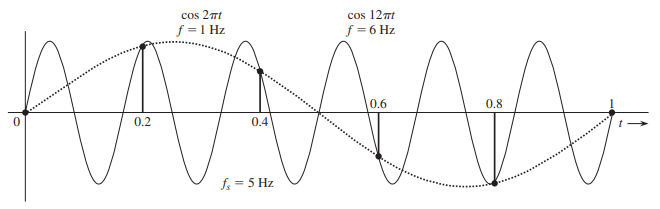
\includegraphics[width=0.9\textwidth]{img/print_aliasing.png}
    \end{center}
    \vspace{-0.5cm}
    \legend{\ABNTEXfontereduzida \textbf{Fonte:} 
    \citeonline[p.~795]{Lathi2018}.}
    

    
    \label{fig:Aliasing}
\end{figure}.

De acordo com o teorema de Nyquist–Shannon onde  $f_s$ é a taxa de amostragem e $f_h$ é a maior frequência a ser processada diz que:


\begin{equation}
    f_s=\frac{1}{T} >2f_h
\end{equation}


Então no exemplo da figura \ref{fig:Aliasing} a taxa de amostragem deveria ser maior do que $12\ Hz$ para que em tempo discreto o sinal de  frequência $6\ Hz$ fosse processada corretamente \cite{Lathi2018}. 






% ####################################################################################
% ####################################################################################
% ####################################################################################
\newpage

\subsection{Conversão analógica-digital}

Um sinal analógico é composto por duas variáveis básicas que são a frequência em Hertz ($Hz$) e a amplitude do sinal em Volts ($v$). Essas duas variáveis podem assumir qualquer valor em uma faixa contínua, ou seja, um sinal analógico pode assumir infinitos valores diferentes de amplitude e de frequência. Já um sinal digital é finito tanto em amplitude e frequência. Se tratando da amplitude, essa pode assumir apenas valores específicos de amplitude chamados de ($L$), que são determinados pela quantidade de bits de resolução ($b$) do conversor A/D \cite{Lathi2018}. 

\begin{equation}\label{eq.conversorAD1}
    2^b = L
\end{equation}

\begin{equation}
    b = \log _{2} L
\end{equation}




Então para converter um sinal analógico em um sinal digital é preciso saber a frequência máxima do sinal a ser medido e utilizar uma taxa de amostragem corretamente como visto na subseção \ref{subsec:Aliasing} e saber a resolução que se deseja ter para a quantização da amplitude do sinal, ou seja, o arredondamento máximo permitido. 





\begin{figure}[ht]
    \centering
    \caption{Onda senoidal quantizada em 4 bits.}
    \begin{center}
        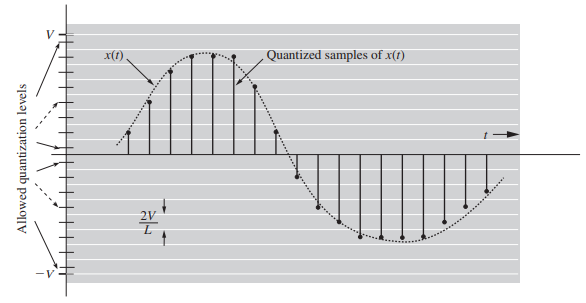
\includegraphics[width=0.9\textwidth]{img/print_Conversao_AD1.png}
    \end{center}
    \vspace{-0.5cm}
    \legend{\ABNTEXfontereduzida \textbf{Fonte:} 
    \citeonline[p.~800]{Lathi2018}.}
    

    
    \label{fig:AD1}
\end{figure}








.

Tendo como exemplo um conversor A/D de $4$ bits, esse possuí $L =2^4= 16$ estados de amplitude diferente. Como mostra o gráfico da figura \ref{fig:AD1}, o sinal analógico foi repartido em 16 níveis de amplitude diferentes e cada nível foi convertido em um código binário como mostra a tabela da figura \ref{fig:AD2}.
 




\begin{figure}[ht]
    \centering
    \caption{Tabela conversão Analógico Digital 4 bits.}
    \begin{center}
        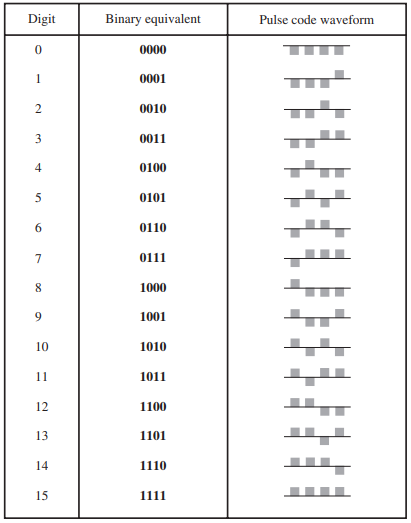
\includegraphics[width=0.5\textwidth]{img/print_Conversao_AD2.png}
    \end{center}
    \vspace{-0.5cm}
    \legend{\ABNTEXfontereduzida \textbf{Fonte:} 
    \citeonline[p.~800*]{Lathi2018}.}
    

    
    \label{fig:AD2}
\end{figure}.


Supondo que a tensão de pico a pico ($VPP$) do sinal fosse de $4 \ v$, então a tensão de entrada do conversor teria de ser no mínimo igual ou maior que $4 \ v$, mas vamos assumir por padrão 5 volts. Utilizando a equação \ref{eq.conversorAD1} se conclui que o conversor apresenta $L=16$ estados de quantização. Então para saber a resolução basta  dividir a tensão máxima por L.

\begin{equation}
    \frac{5 \ v}{2^4}=0,3125 \ v
\end{equation}

Com isso podemos observar que um conversor de 4 bits tem como escala $0,312 \ v$. Caso a aplicação necessitasse medir $0,1 \ v$ esse conversor de 4 bits iria ler como $0 \ v$, substituindo o conversor de 4 bits por um de 8 bits, por exemplo, esse teria uma escala de $0,0195 \ v$ e para medir $0,1V$ iria apresentar um erro de $0,00234 \ v$. Caso esse erro não fosse permitido precisaríamos de um conversor A/D com uma resolução ainda maior \cite{Lathi2018}. 








% ####################################################################################
% ####################################################################################
% ####################################################################################

\newpage

\subsection{Razão sinal-ruído}

Todas as medidas analíticas possuem dois componentes. Um sinal que carrega a informação útil e o outro componente que é formado por informações indesejadas que é chamado de Ruído. A razão sinal ruído, do inglês Signal to Noise Ratio (SNR), é mais usada do que o valor apenas do ruído. Isso porque, o valor SNR indica o quanto de impureza o sinal desejado possuí, como é mostrado no exemplo da figura \ref{fig:RelacaoSinalRuido}a em comparação ao sinal teórico mostrado na figura \ref{fig:RelacaoSinalRuido}b \cite[p.~98]{principioAnaliseInstrumental}.






 




\begin{figure}[ht]
    \centering
    \caption{(a) Efeito do ruído sobre uma medida de corrente contínua de $ 0,9*10^{-15}A$. (b) Média das flutuações.}
    \begin{center}
        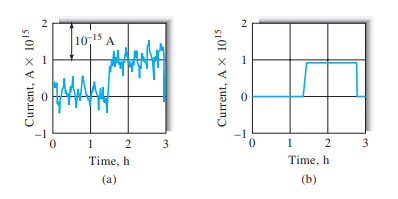
\includegraphics[width=0.7\textwidth]{img/print_relacao_Sinal-Ruido.png}
    \end{center}
    \vspace{-0.5cm}
    \legend{\ABNTEXfontereduzida \textbf{Fonte:} 
    \citeonline[p.~99]{principioAnaliseInstrumental}.}
    

    
    \label{fig:RelacaoSinalRuido}
\end{figure}.
 
 

 
 



A relação sinal ruído é expressa em decibéis. Como se trata de uma escala logarítmica, o SNR é obtido através da seguinte forma: 


\begin{equation}
    P_{sinal,dB}=10 \log(P_{sinal})
\end{equation}



\begin{equation}
    P_{ruído,dB}=10 \log(P_{ruído})
\end{equation}



\begin{equation}
   SNR_{dB} = 10 \log(\frac{P_{sinal}}{P_{ruído}} )
\end{equation}


% ####################################################################################
% ####################################################################################
% ####################################################################################














\newpage



\section {Sensores Inerciais}


 De acordo com a segunda lei de Newton conhecida como princípio fundamental da dinâmica, afirma que a força resultante ($ F $) que atua sobre um corpo é igual ao produto de sua massa ($m$) pela aceleração ($a$). Se rearranjarmos a equação temos:
 
 \begin{equation}
    a = \frac{F}{m}
\end{equation}
 
 Existindo uma relação entre a aceleração, a velocidade ($v$) e a posição ($x$) do objeto por meio de suas derivadas:
  \begin{equation}
    v = f'(x) = \frac{dx}{dt}
\end{equation} 

  \begin{equation}
    a = v'(x) = \frac{d^2x}{dt^2}
\end{equation} 
 
 Apesar de existir essa relação entre as grandezas, a utilização de derivadas em ambientes que contem ruído para se obter a velocidade e a aceleração a partir da derivada da posição terá como resultado erros elevados. Por causa disso, a velocidade e aceleração não são derivadas de sensores de posição, mas sim por sensores inerciais \cite[380]{ModernSensors}.


Os sensores inerciais têm como finalidade a obtenção completa do movimento de um objeto sólido por meio de duas grandezas físicas vetoriais acessíveis que são a aceleração e a velocidade ao redor dos três eixos ortogonais X, Y e Z. Os principais sensores inerciais existentes são os acelerômetros utilizados para se obter a aceleração em $a  = m/s^2$ e os giroscópios utilizados para obtenção das velocidades angulares em $\omega= rad/s $ \cite[p.~527]{Korvink2006}.




% ####################################################################################
% ####################################################################################
% ####################################################################################


%#############################################
%  Esta Pronto     v
%#############################################



\newpage
\subsection{Acelerômetro}


Os acelerômetros lineares pertencem à classe dos sensores inerciais que não requerem
referência a um sistema de coordenadas estacionário. Normalmente se utiliza três acelerômetros ortogonais com o intuito de medir a aceleração linear em cada eixo do espaço incluindo a gravidade. Assim, um acelerômetro típico deve responder a várias formas de acelerações desde movimento lentos, fortes a impactos e vibrações. Um fato interessante é que ao processar os sinais desses dispositivos é possível rastrear a posição e orientação de um objeto em movimento \cite{ModernSensors}.

 Os acelerômetros mecânicos consistem em um sistema massa-mola com um sensor de deslocamento interno como mostra a figura \ref{fig:ModernSensors}a. Como a massa de prova ($m$), a constante elástica da mola ($k$), e o valor do deslocamento ($\Delta x$)  provocado pela aceleração são conhecidos, a obtenção do valor da aceleração se torna possível utilizando as equações de Hooke e a segunda lei de Newton.


\begin{equation}
    F = -k\cdot\Delta x
\end{equation}


\begin{equation}
    a =\frac{-k\cdot\Delta x}{m}
\end{equation}


 

\begin{figure}[ht]
    \centering
    \caption{(a) Conceito de acelerômetro mecânico linear. (b) Diagramas de tempo.}
    \begin{center}
        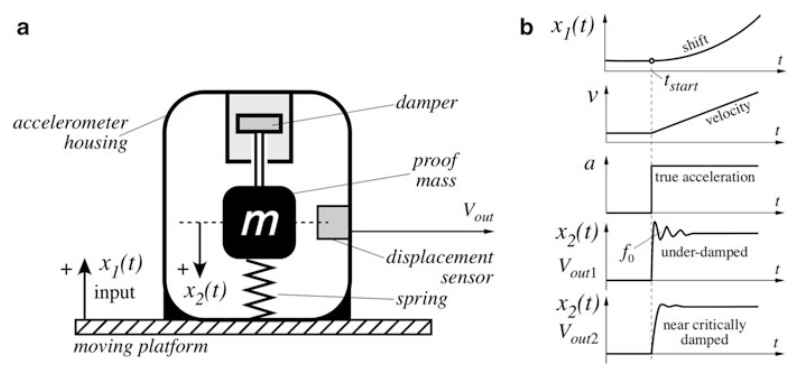
\includegraphics[width=1\textwidth]{img/print_acelerometro_conceito.png}
    \end{center}
    \vspace{-0.5cm}
    \legend{\ABNTEXfontereduzida \textbf{Fonte:} 
    \citeonline[p.~393]{ModernSensors}.}
    

    
    \label{fig:ModernSensors}
\end{figure}.
\newpage



 Um bom acelerômetro deve ter dois parâmetros bem identificados que são a frequência ressonante ou frequência natural e uma faixa de resposta de frequência plana onde a medição da aceleração se torna mais precisa sem distorções provocadas pelas características de frequência do
acelerômetro como é mostrado na figura \ref{fig:grafico_acelerometro}. No entanto, quando a frequência medida é muito maior do que o limite de largura de banda de operação do acelerômetro, um filtro passa-baixa é necessário para filtrar o sinal \cite{ModernSensors}.
 
 
 



\begin{figure}[ht]
    \centering
    \caption{Uma frequência-resposta de um acelerômetro onde f\textsubscript{0} é a frequência natural e f\textsubscript{ref} é a frequência de referência.}
    \begin{center}
        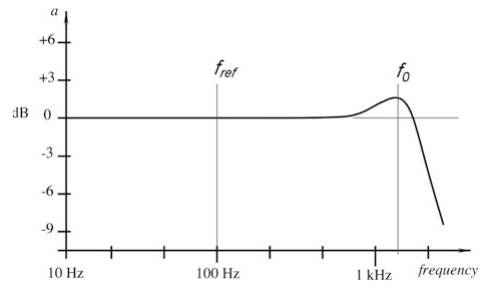
\includegraphics[width=0.7\textwidth]{img/print_grafico_resposta_do_acelerometro.png}
    \end{center}
    \vspace{-0.5cm}
    \legend{\ABNTEXfontereduzida \textbf{Fonte:} 
    \citeonline[p.~396]{ModernSensors}.}
    

    
    \label{fig:grafico_acelerometro}
\end{figure}.

%#############################################
%  Esta Pronto     ^
%#############################################










Como o sistema apresenta uma massa, uma  mola e um amortecedor interno, com a finalidade de consumir a energia fornecida a mola pela aceleração, fazendo com que a massa volte a sua posição inicial (sem aceleração). O sistema irá se comportar como um oscilador, tendo características estáticas e dinâmicas. Uma das características estáticas mais importantes é a sensibilidade estática (S) dada por:


\begin{equation}
    S=\frac{m}{k} = \frac{1}{\omega_0^2} = \frac{1}{(2 \pi f_0)^2}
    \label{9.19_equacao_sensibilidade_estatica}
\end{equation} 

Onde o S é inversamente proporcional ao quadrado da frequência natural ($f_0$) em Hz. Outra característica estática é o coeficiente de amortecimento b que é definido através do parâmetro $\zeta$ chamado de razão de amortecimento

\begin{equation}
    b = 2 \zeta\sqrt{km}   
    \label{9.21_equacao_coeficiente_amortecimento}
\end{equation} 




Levando em conta todas as forças que atuam na massa de prova (força de inércia, força da mola, e amortecimento) a equação diferencial linear de segunda ordem que descreve esse sistema é:


\begin{equation}
    m\frac{d^2x_2}{dt^2}+b(\frac{dx_2}{dt}-\frac{dx_1}{dt})+k(x_2-x_1)=0
    \label{9.22_equacao_diferencial}
\end{equation} 


Chamando $ x_2 - x_1 = \Delta x $ que é o deslocamento relativo da massa de prova sendo traduzida pelo sensor de deslocamento como uma tensão de saída V\textsubscript{out}. Então, a equação \ref{9.22_equacao_diferencial} pode ser reescrito como

  \begin{equation}
    m\frac{d^2\Delta x}{dt^2}+b\frac{d\Delta x}{dt}+k\Delta x=-ma=-F
    \label{9.23_equacao_diferencial}
\end{equation} 


Tendo como solução da equação \ref{9.23_equacao_diferencial} para um deslocamento relativo $\Delta x(t)$ :


\begin{equation}
    \Delta x(t) = Be^{-\zeta\sqrt{t\frac{k}{m}}}\sin{(2\pi f_dt+\varphi )}  - Sa 
    \label{9.24_equacao}
\end{equation} 





Onde o fator B e o deslocamento de fase $\varphi$, dependem da posição da massa de prova no
momento do início da aceleração.
A frequência amortecida $f_d$ é diferente da frequência natural $f0$ e só é valida para $\zeta<1$ definida como:


\begin{equation}
    f_d = f0\sqrt{1-\zeta^2} 
    \label{9.25_equacao}
\end{equation} 


Várias conclusões podem ser tiradas da solução \ref{9.24_equacao}, como a saída ter uma
natureza oscilatória decadente caracterizada pela primeira soma, sendo que a taxa de decaimento é exponencial com uma constante de tempo:


\begin{equation}
    \tau = \frac{1}{\zeta}\sqrt{\frac{m}{k}}
    \label{9.26_equacao_Constante_tempo}
\end{equation} 


É observável que pela equação \ref{9.26_equacao_Constante_tempo}, quanto maior a razão de amortecimento $\zeta$, mais rápido as oscilações indesejadas desaparecem. Porém, a medida que $\zeta$  fica maior que 1, o acelerômetro fica menos sensível e consequentemente mais lento. A melhor condição é quando ($\zeta \approx 1$), apresentando uma resposta crítica ou quase criticamente amortecida se comportando da forma mais aproximada da verdadeira aceleração como é mostrado no gráfico de $V_{out2}$ da figura \ref{fig:ModernSensors}b \cite{ModernSensors}. 


Vale ressaltar que a sensibilidade de um acelerômetro é a razão de uma saída elétrica para a entrada mecânica, expresso em volts por unidade de aceleração. Por exemplo, a sensibilidade pode ser especificada como $1 V/g$ (unidade de aceleração: $ g = 9,806 \ m/s^2$ ao nível do mar. Ela é tipicamente medida em uma única frequência de referência na forma de onda senoidal \cite{Korvink2006}.


\newpage











% ####################################################################################
% ####################################################################################
% ####################################################################################


\subsection{Giroscópio}


 

Os giroscópios pertencem à classe dos sensores rotativos inerciais. Este sensor é um dispositivo responsável por "guardar a direção", isso significa que ele produz um sinal na saída sempre que a velocidade angular se desvia de zero, o que acontece quando a plataforma começa a girar. O funcionamento do giroscópio tem como base o princípio fundamental da conservação do momento angular, que diz que em qualquer sistema de partículas, o momento angular total do sistema em relação a qualquer ponto fixo no espaço permanece constante, desde que nenhuma força externa aja sobre o sistema. Um sensor inercial rotativo completo normalmente contém três giroscópios de taxa ortogonal, medindo as velocidades angulares em cada eixo. \cite{ModernSensors}. 

Um giroscópio mecânico é composto por um disco maciço livre para girar em torno de um eixo de rotação, que está confinado dentro de uma estrutura que é livre para girar em torno de um ou dois eixos como mostra a figura \ref{fig:Giroscopio_Conceitual}. Assim, dependendo do número de eixos rotativos, um giroscópio pode ser de um ou dois graus de liberdade. 


 


\begin{figure}[ht]
    \centering
    \caption{Giroscópio mecânico conceitual.}
    \begin{center}
        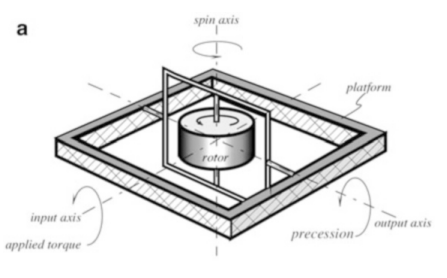
\includegraphics[width=0.8\textwidth]{img/print_giroscopio_mecanico_conceitual.png}
    \end{center}
    \vspace{-0.5cm}
    \legend{\ABNTEXfontereduzida \textbf{Fonte:} 
    \citeonline[p.~386]{ModernSensors}.}
    

    
    \label{fig:Giroscopio_Conceitual}
\end{figure}.



Esse dispositivo inercial rotativo, pode ser feito para fornecer um torque (ou sinal de saída) que é proporcional a velocidade angular em torno de um eixo perpendicular ao eixo de rotação.
Quando o rotor gira livremente, ele tende a preservar sua posição axial. Se a plataforma do giroscópio gira em torno do eixo de entrada, o giroscópio desenvolverá um torque em torno de um eixo perpendicular (saída), girando assim, seu eixo de rotação em torno do eixo de saída. Esse fenômeno é chamado de precessão de um giroscópio, e isso pode ser explicado pela lei de Newton do movimento para rotação, onde a taxa de tempo de mudança do momento angular sobre qualquer eixo é igual ao torque aplicado em torno do eixo dado. Ou seja, quando um torque T é aplicado em torno do eixo de entrada, e a velocidade $\omega$ do rotor é mantida constante, o momento angular do rotor pode ser alterado apenas girando a projeção do eixo de rotação em relação ao eixo de entrada. 


\begin{equation}
    T = I\omega \Omega
    \label{equação_9.10}
\end{equation}


Como mostra a equação \ref{equação_9.10}, a taxa de rotação do eixo de rotação em torno do eixo de saída é proporcional ao torque aplicado, onde $\Omega$ é a velocidade angular sobre o eixo de saída e I é a inércia de um giroscópio em torno do eixo de rotação. Se tratando da precisão de um giroscópio mecânico, esta depende muito dos efeitos que podem causar torques adicionais indesejados que pode causar desvios. As fontes destes problemas são o atrito, rotor desbalanceado, efeitos magnéticos, etc \cite{ModernSensors}.

Outros métodos para detectar uma direção e velocidade angular foram desenvolvidos, por exemplo, o Sistema de Posicionamento Global (GPS), mas, ele simplesmente não pode ser empregado no espaço, debaixo d'água, em túneis, dentro de prédios, ou sempre que o tamanho e custo forem de uma importância primordial. Além disso, a resolução espacial do GPS quase não é suficiente para muitos dispositivos  e isso torna o uso de um giroscópio bastante relevante principalmente em mísseis e foguetes \cite{Korvink2006}. 














% ####################################################################################
% ####################################################################################
% ####################################################################################


\section{Magnetômetro}


O sensor magnetômetro atua como uma bússola digital sendo utilizado para aferir a intensidade, direção e sentido de campos magnéticos em sua proximidade. Na ausência de campos eletromagnéticos locais fortes, essas medições serão do ambiente, no caso, detectando o campo magnético da Terra e permitindo assim que o sensor determine a sua direção em relação ao Polo Norte geomagnético. Vale lembrar que a  direção geomagnética e a verdadeira direção em relação ao Polo Norte geográfico pode variar por várias dezenas de graus, dependendo da localização no planeta. Normalmente esse tipo de sensor retorna a intensidade do campo eletromagnético em Microtesla ($\micro T$), nas três coordenadas X,Y e Z \cite{Jepson2011}.

\newpage







% ####################################################################################
% ####################################################################################
% ####################################################################################







% ####################################################################################
% ####################################################################################
% ####################################################################################









% ####################################################################################
% ####################################################################################
% ####################################################################################
\newpage
\section {INSTRUMENTAÇÃO ELETRÔNICA}



\subsection{Sensor BNO055}\label{subsec:BNO055}



O BNO055 é um System in Package (SiP), desenvolvido pela empresa BOSCH. Esse circuito integrado contém um acelerômetro triaxial de 14 bits de resolução, um Giroscópio de 16 bits de resolução com alcance de ±2000 graus por segundo, um sensor geomagnético triaxial e um microcontrolador córtex M0+ de 32 bits executando o software de fusão de sensores Bosch Sensortec, que é responsável por corrigir e integrar as informações dos 3 sensores em um único encapsulamento \cite{BOSCH2021}.  


 

\begin{figure}[ht]
    \centering
    \caption{Sensor BNO055 com os circuitos adicionais.}
    \begin{center}
        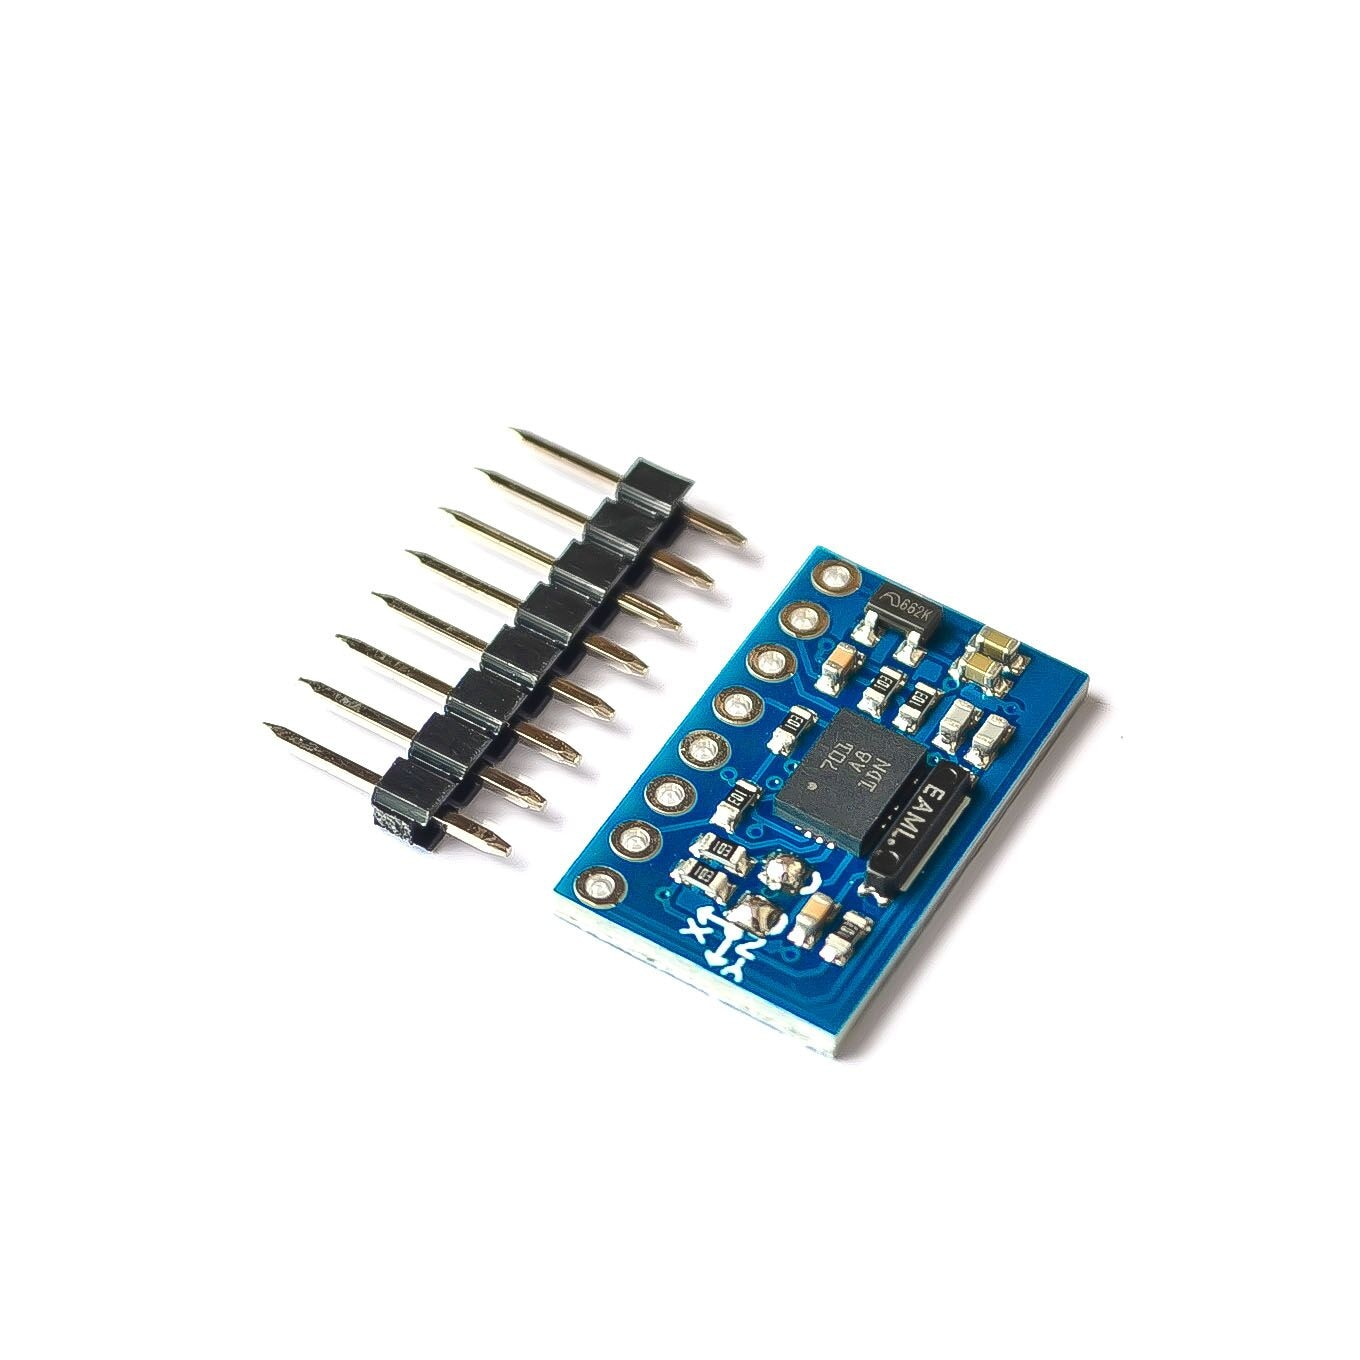
\includegraphics[width=0.50\textwidth]{img/Sensor BNO055.jpg}
    \end{center}
    \vspace{-0.5cm}
    \legend{\ABNTEXfontereduzida \textbf{Fonte: Site Aliexpress}}
    \label{fig:BNO055}
\end{figure}.




O  Circuito Integrado CI montado no modulo da figura \ref{fig:BNO055} possui quatro vantagens em relação a utilização de três sensores separados:


 \begin{enumerate}
   \item Redução de espaço e peso adicionado ao foguete;
   \item Redução de processamento do microcontrolador principal;
   \item Redução de falhas de comunicação devido a redução de componentes eletrônicos na placa de circuito impresso PCB;
   \item Redução da complexidade de desenvolvimento de software e hardware.
 \end{enumerate}


















% ####################################################################################
% ####################################################################################
\newpage
\subsection{Sensor BME280}


O BME280 é um sensor três em um desenvolvido pela empresa BOSCH. Esse dispositivo apresenta um sensor de pressão atmosférico com range de $300$ à $1100 \ hPa$, um sensor de umidade com range de $0$ à $100\% $ umidade relativa e um sensor de temperatura com range de $-40$ à $+85 \ \celsius$ \cite{BMP280}.

\begin{equation}
    P = \rho gh
     \label{equação_10}
\end{equation}


De acordo com a equação \ref{equação_10}, onde $P = pressão$, $\rho =  densidade \ do \ ar$ e $h = altura $. É observável que a densidade do ar interfere na pressão medida, de acordo com a lei dos gases, a temperatura e umidade interferem na densidade do gases, logo o sensor BME280 visto na figura \ref{fig:BMP280} se torna um altímetro mais preciso do que o BMP280  que só conta com o sensor de pressão atmosférica e consequentemente não pode corrigir os efeitos causados na pressão pela temperatura e umidade do ar  \cite[p.~465]{Halliday2010}.




 



\begin{figure}[ht]
    \centering
    \caption{Sensor BME280 com os circuitos adicionais.}
    \begin{center}
        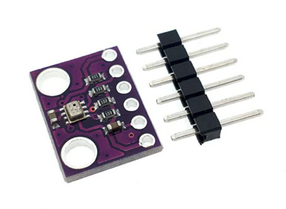
\includegraphics[width=0.50\textwidth]{img/BMP280.png}
    \end{center}
    \vspace{-0.5cm}
    \legend{\ABNTEXfontereduzida \textbf{Fonte: Site Aliexpress}}
    %\citeonline{BNO055}.}
    \label{fig:BMP280}
\end{figure}.

Assim como o sensor BNO055 apresentado na subseção \ref{subsec:BNO055},  o  Circuito Integrado CI montado no modulo da figura \ref{fig:BMP280} possui vantagens em relação a utilização de três sensores separados:


 \begin{enumerate}
   \item Redução de espaço e peso adicionado ao foguete;
   \item Redução de falhas de comunicação devido a redução de componentes eletrônicos na placa de circuito impresso PCB;
   \item Redução da complexidade de desenvolvimento de hardware.
 \end{enumerate}






% ####################################################################################
% ####################################################################################
\newpage
\subsection{GPS NEO-6M}

O modulo NEO-6M é um sistema de posicionamento Global (GPS) que tem suporte até 50 canais de satélites geoestacionários, taxa de navegação máxima até $5 \ Hz$, precisão horizontal de $2,5 \ m$ e podendo operar em uma faixa de $-40$ à $+80 \ \celsius$  \cite{NEO-6M}. Esse modulo por padrão retorna o seguinte protocolo NMEA de mensagens:
 \begin{enumerate}
    \item GSV = O número de satélites disponíveis, o número de identificação por satélite, elevação, azimute e valores SNR.
    \item RMC = Dados de hora, data, posição, curso e velocidade. 
    \item GSA = Modo de operação do receptor GPS, satélites usados na solução de posição,"' e valores DOP.
    \item GGA = Dados de tempo, posição e correção dos dados.
    \item GLL = Latitude, longitude, tempo UTC de correção de posição e status 
    \item VTG = Informações de curso e velocidade relativas ao solo.
 \end{enumerate}



Como mostra a figura \ref{fig:GPSNEO6M}, este modulo por ser pequeno e leve tem a vantagem de não impactar demasiadamente no desempenho do foguete. Vale destacar que apesar deste modulo apresentar uma taxa de atualização baixa na ordem de $5 \ Hz$, não é tão relevante para o projeto adicionar um GPS com uma taxa de atualização mais alta como é o caso do NEO-7M com taxa de $10 \ Hz$ ou NEO-8M com taxa de $15 \ Hz$ e consequentemente aumentar o custo do projeto, já que sua função principal é ajudar na localização do foguete. 


 



\begin{figure}[ht]
    \centering
    \caption{GPS NEO-6M com os circuitos adicionais e antena.}
    \begin{center}
        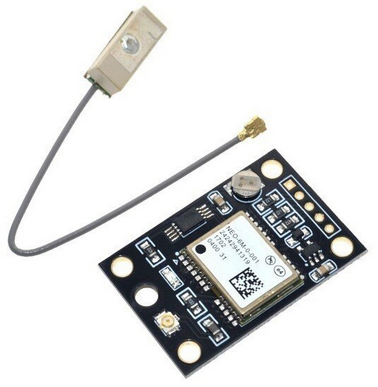
\includegraphics[width=0.40\textwidth]{img/NEO-6M GPS.png}
    \end{center}
    \vspace{-0.5cm}
    \legend{\ABNTEXfontereduzida \textbf{Fonte: Site Aliexpress}}
    %\citeonline{BNO055}.}
    \label{fig:GPSNEO6M}
\end{figure}.















\begin{comment}
Este é um comentário de múltiplas linhas.
Com certeza útil para esconder partes grandes de texto ainda não revisadas.
Ou para encontrar um problema do seu código LaTeX que não compila.






\alpha α
\beta β
\gamma e \Gamma γ e Γ
\delta e \Delta δ e ∆
\epsilon e \varepsilon ǫ e ε
\zeta ζ
\eta η
\vartheta, \theta e \Theta θ, θ e Θ
\iota ι
\kappa κ
\lambda e \Lambda λ e Λ
\mu μ
\nu ν
\xi e \Xi ξ e Ξ
\pi e \Pi π e Π
\rho e \varrho ρ e ̺
\sigma, \varsigma e \Sigma σ, ς e Σ
\tau τ
\upsilon e \Upsilon υ e Υ
\phi, \varphi e \Phi φ, φ e Φ
\chi χ
\psi e \Psi ψ e Ψ
\omega e \Omega ω e Ω




\end{comment}









% ####################################################################################
% ####################################################################################
% ####################################################################################
\newpage
\subsection{Radio Lora^{TM}}




% ###############################################

O modulo de rádio frequência RF lora é uma boa escolha devido as suas características benéficas como uma taxa de transferência variável o que possibilita a troca de largura de banda por alcance e também pelo seu custo benefício. Por padrão ele apresenta uma taxa de transferência de dados de $2,4 \ kbps$ o que é mais do que suficiente para transmitir os dados dos sensores do foguete para o solo \cite{EBYTE2019}. 

Como mostra a figura \ref{fig:RadioLora} esse modulo é relativamente pequeno e leve, se tornando uma escolha ideal por não interferir no desempenho do foguete. Além disso, segundo o datasheet o modulo pode atingir um alcance de até $8 \ km$ o que significa que poderá suprir as necessidades tanto de foguetemodelos de porte iniciante e intermediário.






\begin{figure}[ht]
    \centering
    \caption{Radio Lora E32-433T30D.}
    \begin{center}
        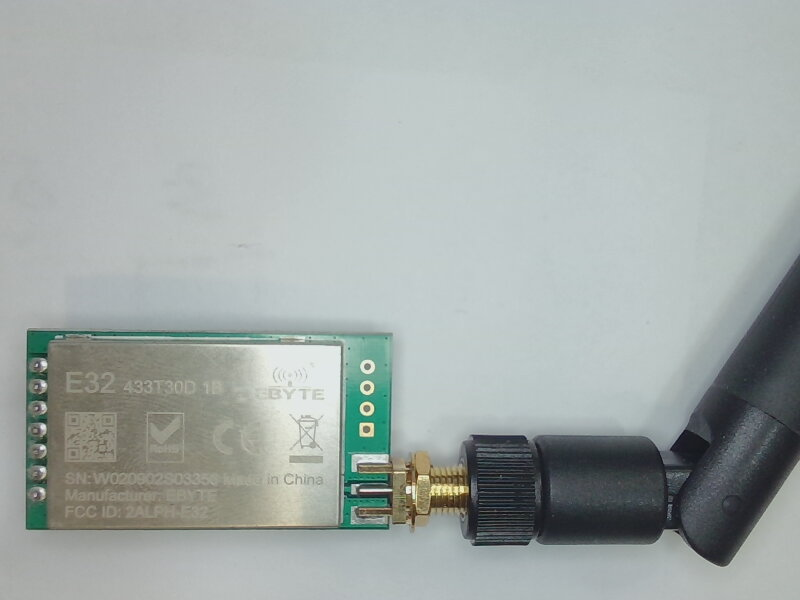
\includegraphics[width=0.6\textwidth]{img/Modulo RF Lora.jpg}
    \end{center}
    \vspace{-0.5cm}
    \legend{\ABNTEXfontereduzida \textbf{Fonte: O autor.} 
    }
   \label{fig:RadioLora}
\end{figure}

% ###############################################
Como mostra a tabela \ref{tab:radioLora} retirado do datasheet é possível ver as principais características do modulo entre elas a frequência de transmissão trabalhando dentro de $410 \ MHz$ até $441 \ MHz$, por padrão $433 \ MHz$, que é uma frequência de grande interesse já que ela não sofre tamanha interferência causada por inúmeros outros dispositivos operando na mesma faixa de frequência como é o caso de aparelhos em $2,4 GHz$.



\begin{table}[!htb]
	\centering
	\caption{\label{tab:radioLora} Especificações do Modulo E32- 433T30D.}
	\begin{adjustbox}{max width=\textwidth}
%		\begin{tabular}{@{} p{5cm} |c|c|c|c|@{}}
        \begin{tabular}{@{} p{2cm} |c|c|c|c|c|c}
		\toprule
		\textbf{Model} & \textbf{Core IC} & \textbf{Frequency Hz} & \textbf{Tx Power dBm} & \textbf{Distance km} & \textbf{Date Rate} & \textbf{Interfece}\\ \hline

		\textbf{E32- 433T30D} &
			SX1278 & 433M & 30 & 8 & 0.3k~19.2k & SMA-K
%		\\ \hline

		\\ \bottomrule
	\end{tabular}
	\end{adjustbox}
	\legend{\textbf{Fonte:} \citeonline[p.~17]{EBYTE2019}}
\end{table}









% ####################################################################################
% ####################################################################################
% ####################################################################################

\newpage
%\section{Seção de exemplo 1 - Como fazer citações}
\begin{comment}
Existem vários tipos de citações...
















%\imagem{0.15}{missil_balistico_V2}{Missil balistico V2 sendo preparado para lançamento em %Cuxhaven, na Alemanha, 15 de  outubro de 1945.}{AP IMAGES, 2022}

%A figura \ref{img:missil_balistico_V2} é um exemplo do outro tipo de figura abordada aqui, chamada %de figura composta. Esta figura é composta de outras subfiguras.



%\begin{figure}[!htb]
%\centering
 %   \caption{\label{img:missil_balistico_V2} Missil balistico V2 sendo preparado para lançamento em Cuxhaven, na Alemanha, 15 de  outubro de 1945.}

  %  \legend{\textbf{Fonte:AP IMAGES, 2022}\citeonline{ACESSADO EM: https://www.apimages.com/metadata/Index/Watchf-AP-I-DEU-APHSL37937-Post-WWII-germany-V2-/e918f669900d409caba6ccabee822d81/100/0}}
%\label{fig:dag}
%\end{figure}





%\begin{figure}[!htb]
%\centering
 %   \caption{\label{img:figura1} Exemplo de figura composta}
  %  \subcaptionbox{\label{img:subfigura1} Subfigura 1}{
\includegraphics[scale=.1]{img/placeholder}}\qquad
   % \subcaptionbox{\label{img:subfigura2} Subfigura 2}{
\includegraphics[scale=.1]{img/placeholder}}
%    \vspace{1.5em}
%    \legend{\textbf{Fonte:} \citeonline{SUA-REFERENCIA}}
%\label{fig:dag}
%\end{figure}




Para referenciar uma figura deve ser usada comando \textbackslash ref\{img:<label ou nome do arquivo>\}, como exemplo, estamos referenciando a figura \ref{img:placeholder}. Isso vale tanto para figuras simples quanto para as compostas, como por exemplo as figuras \ref{img:subfigura1} e \ref{img:subfigura2}. Ao inserir uma figura, ela é automaticamente identificada e incluída no elemento pré-textual da lista de figuras.





%\lipsum[5-10]

Colocar citações longas entre \textbackslash begin\{citacao\} e \textbackslash end\{citacao\}, exemplo: 

\begin{citacao}
``\lipsum[1]''

\cite{REFERENCIA}
\end{citacao}





\section{Seção de exemplo 2 - Como inserir figuras}

Neste trabalho iremos exemplificar duas formas de se inserir figuras no Latex. O primeiro método insere, no documento, uma figura simples por meio do comando:

\textbackslash imagem\{ Escala \}\{ Arquivo sem extensão \}\{ Descrição \}\{ Fonte \}

\textbf{Obs.:} A fonte pode ser uma citação do tipo  \textbackslash citeonline\{\}.

A figura \ref{img:placeholder} é um exemplo deste método.

%--------------------------------------------------------------------------------------
% Esse é um exemplo de figura simples
%--------------------------------------------------------------------------------------
\imagem{0.15}{placeholder}{Uma figura simples}{O autor}

A figura \ref{img:figura1} é um exemplo do outro tipo de figura abordada aqui, chamada de figura composta. Esta figura é composta de outras subfiguras.
%--------------------------------------------------------------------------------------
% Esse é um exemplo de figura composta de outras subfiguras
%--------------------------------------------------------------------------------------
\begin{figure}[!htb]
\centering
    \caption{\label{img:figura1} Exemplo de figura composta}
    \subcaptionbox{\label{img:subfigura1} Subfigura 1}{
\includegraphics[scale=.1]{img/placeholder}}\qquad
    \subcaptionbox{\label{img:subfigura2} Subfigura 2}{
\includegraphics[scale=.1]{img/placeholder}}
    \vspace{1.5em}
    \legend{\textbf{Fonte:} \citeonline{SUA-REFERENCIA}}
\label{fig:dag}
\end{figure}

%\begin{figure}[!htb]
%\centering
%    \caption{\label{img:telas} Telas da aplicação cliente}
%    \subcaptionbox{\label{img:inicial} Abertura}{\includegraphics[scale=.12]{img/APP/inicial}}\qquad
%    \subcaptionbox{\label{img:login} \textit{Login}}{\includegraphics[scale=.12]{img/APP/login}}\qquad
%    \subcaptionbox{\label{img:cadastro} Cadastro}{\includegraphics[scale=.12]{img/APP/cadastro}}\qquad
%    \subcaptionbox{\label{img:hist-rel}Sobre}{\includegraphics[scale=.12]{img/APP/sobre}}\\
%    \vspace{1.5em}
%    \subcaptionbox{\label{img:dados_atuais}Dados atuais}{\includegraphics[scale=.15]{img/APP/atual}}\qquad
%    \subcaptionbox{\label{img:hist-time}Seleção de período}{\includegraphics[scale=.15]{img/APP/periodo}}\qquad
%    \subcaptionbox{\label{img:hist-rel}Exibir histórico}{\includegraphics[scale=.15]{img/APP/historico}}\\
%    \vspace{2.5em}
%    \legend{\textbf{Fonte:} O Autor}
%\label{fig:dag}
%\end{figure}

Para referenciar uma figura deve ser usada comando \textbackslash ref\{img:<label ou nome do arquivo>\}, como exemplo, estamos referenciando a figura \ref{img:placeholder}. Isso vale tanto para figuras simples quanto para as compostas, como por exemplo as figuras \ref{img:subfigura1} e \ref{img:subfigura2}. Ao inserir uma figura, ela é automaticamente identificada e incluída no elemento pré-textual da lista de figuras.




\section{Seção de exemplo 3 - Sobre tabelas}

As tabelas em Latex são deveras capciosas, por isso não serão abordadas em sua completude neste documento.

Há um site que possui uma ferramenta interessante para ser utilizada na construção tabelas em Latex.

\centerline{\href{https://www.tablesgenerator.com/}{ O Tables Generator } <-- Isto é um \textit{link} :D}

Contudo, busquem entendimento sobre o assunto, pois tabelas são elementos textuais importantes e enriquecem muito o texto, quando bem construídas.

A tabela \ref{tab:crossplatform} é um exemplo de como uma tabela pode ser construída, assim como a tabela do anexo \ref{anex:anexo1}.

\begin{table}[!htb]
	\centering
	\caption{\label{tab:crossplatform} Tipos de aplicações e abordagens preferenciais.}
	\begin{adjustbox}{max width=\textwidth}
		\begin{tabular}{@{} p{5cm} |c|c|c| @{}}
		\toprule
		\textbf{Código da Aplicação} & \textbf{Web} & \textbf{Híbrida} & \textbf{Interpretada / Compilação Cruzada} \\ \hline

		\textbf{Aplicações baseadas em dados providos por um servidor} &
			3 & 2 & 1
		\\ \hline

		\textbf{Aplicações independentes} & 1 & 2 & 3\\ \hline

		\textbf{Aplicações baseadas em sensores e processamento de dados no dispositivo} & 1 & 2 & 3\\ \hline

		\textbf{Aplicações baseadas em sensores e processamento de dados no servidor} & 1 & 3 & 2\\ \hline

		\textbf{Aplicações Cliente-Servidor} & 1 & 3 & 2 \\ \bottomrule
	\end{tabular}
	\end{adjustbox}
	\legend{\textbf{Fonte:} \citeonline{raj2012study} (Traduzido)}
\end{table}

Também é possível criar quadros, que são ligeiramente diferente de tabelas. Acompanhe o exemplo no Quadro \ref{qua:confusionmatrix}

\begin{quadro}
	\centering
	\caption{\label{qua:confusionmatrix}Exemplo de matriz de confusão}
	\begin{tabular}{ll|c|c|}
		\cline{3-4}
		\multicolumn{1}{c}{\textbf{}} & \multicolumn{1}{c|}{\textbf{}} & \multicolumn{2}{l|}{\textbf{Classe prevista}} \\ \cline{3-4}
		 & \multicolumn{1}{c|}{\textbf{}} & Classe = 1 & Classe = 0 \\ \hline
		\multicolumn{1}{|l|}{\multirow{2}{*}{\textbf{Classe real}}} & Classe = 1 & $f_{11}$ & $f_{10}$ \\ \cline{2-4}
		\multicolumn{1}{|l|}{} & Classe = 0 & $f_{01}$ & $f_{00}$ \\ \hline
	\end{tabular}
	\Ididthis
\end{quadro}


\begin{quadro}
	\caption{\label{qua:cron}Cronograma}
	\center
	\begin{tabular}{|c|c|c|c|c|c|}
	\hline
	\multicolumn{1}{|l|}{Atividade} & \multicolumn{1}{l|}{Set/19} & \multicolumn{1}{l|}{Out/19} & \multicolumn{1}{l|}{Nov/19} & \multicolumn{1}{l|}{Dez/19} & \multicolumn{1}{l|}{Jan/20} \\ \hline
	1                               & x                           &                             &                             &                             &                             \\ \hline
	2                               &                             & x                           &                             &                             &                             \\ \hline
	3                               &                             & x                           &                             &                             &                             \\ \hline
	4                               &                             &                             & x                           & x                           &                             \\ \hline
	5                               &                             & x                           & x                           & x                           &                             \\ \hline
	6                               &                             &                             &                             &                             & x                           \\ \hline
	
	\end{tabular}
	\legend{\textbf{Fonte:} Elaborado pela autora (2019)}
	\end{quadro}

\section{Subseção de exemplo 4 - Seções}



\end{comment}
		%--------------------------------------------------------------------------------------
% Este arquivo contém a sua metodologia
%--------------------------------------------------------------------------------------
\chapter{Materiais e Métodos} \label{ch:MM} %Uma label é como você referencia uma seção no texto com a tag \ref{}


\section{Arquitetura do Sistema embarcado do foguete} 

Com o intuito de capturar as principais grandezas produzidas pelo minifoguete e reduzir a massa e o volume ocupado pelo sistema, foi escolhido sensores capazes de mensurar mais de uma variável em um único encapsulamento e assim reduzir a necessidade de vários sensores separados. 

O microcontrolador foi escolhido tomando como base um custo-benefício melhor do que o atmega328p, que é bastante popular na plataforma arduino. Na data 05/04/2022, esse microcontrolador pode ser encontrado na loja Aliexpress por $47,31$ reais, já o STM32f103C8T6 por $36,47$. Além da redução de custo, o microcontrolador escolhido apresenta dez vezes mais memória SRAM, mais periféricos, processamento em $32 \ bits$ contra $8 \ bits$ e execução das instruções com clock de $72 \ MHz$ contra $16 \ MHz$ do atmega328p. 

Por fim, o rádio selecionado foi o modulo Lora, por apresentar um baixo custo e possuir um longo alcance de até $8 \ km$, possibilitando assim, seu uso em minifoguetes avançados. Com esses componentes escolhidos, foi projetado o diagrama mostrado na figura \ref{fig:Fluxograma_Sistema1}, que representa um sistema simples de entrada de dados através dos sensores, pre-processamento desses dados pelo microcontrolador e por fim a saída através da gravação em um cartão micro SD e o envio pelo rádio.



 


\begin{figure}[ht]
    \centering
    \caption{Diagrama sistema embarcado do minifoguete.}
    \begin{center}
        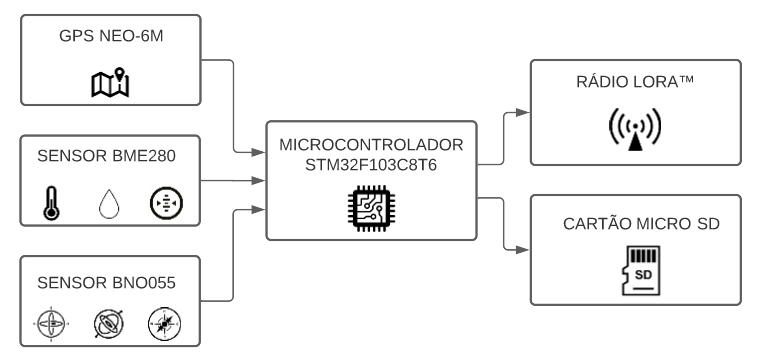
\includegraphics[width=1.0\textwidth]{img/Fluxograma_Sistema1.png}
    \end{center}
    \vspace{-0.5cm}
    \legend{\ABNTEXfontereduzida \textbf{Fonte: O autor.}}
    %\citeonline{BNO055}.}
    \label{fig:Fluxograma_Sistema1}
\end{figure}.





\section{Arquitetura do Sistema embarcado receptor } 

O sistema receptor é mais simples do que o sistema transmissor contido no foguete, porque, a única função desse sistema é repassar os dados recebidos do foguete para o computador. Como mostra o diagrama da figura \ref{fig:Fluxograma_Sistema2}, esse sistema possui apenas um modulo de rádio Lora na configuração receptor e um microcontrolador responsável por comunicar com o computador.





 



\begin{figure}[ht]
    \centering
    \caption{Diagrama sistema em solo.}
    \begin{center}
        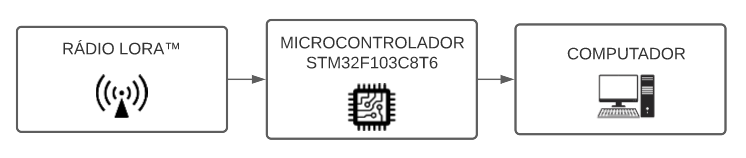
\includegraphics[width=1.0\textwidth]{img/Fluxograma_Sistema2.png}
    \end{center}
    \vspace{-0.5cm}
    \legend{\ABNTEXfontereduzida \textbf{Fonte: O autor.}}
    %\citeonline{BNO055}.}
    \label{fig:Fluxograma_Sistema2}
\end{figure}.
 

 
 
%######################################################################################## 
%######################################################################################## 
%######################################################################################## 

\section{Firmware} 



%####################################################################
%####################################################################
%####################################################################



Como o sistema a ser projetado tem a finalidade de obter dados de um objeto com altas velocidades. É de extrema importância conhecer os limites impostos por  componente, e assim, projetar um firmware capaz de extrair o máximo de cada componente. Com base no datasheet de cada sensor foi possível obter a taxa de atualização máxima e montar a tabela \ref{tempoderesposta_sensores}. 





\begin{table}[!thb]
	\centering
	\caption{\label{tempoderesposta_sensores}Tempo de resposta máxima dos sensores}
	\begin{tabular}{ll|c|c|}
		\cline{3-4}
		\multicolumn{1}{c}{\textbf{}} & 
		\multicolumn{1}{c|}{\textbf{}} & 
		\multicolumn{2}{l|}{\textbf{Taxa de atualização}} 
		\\ \cline{3-4}
		 & \multicolumn{1}{c|}{\textbf{}} & Hertz   & Milissegundos
		\\ \hline
		\multicolumn{1}{|c|}{\multirow{3}{*}{\textbf{Sensor BNO055}}} & Acelerômetro & $100$ & $10$ 
		\\ \cline{2-4}
		\multicolumn{1}{|l|}{} & Giroscópio & $100$ & $10$ 
		\\ \cline{2-4}
	    \multicolumn{1}{|l|}{} & Magnetrômetro & $20$ & $50$ 
		\\ \hline
		\multicolumn{1}{|c|}{\multirow{3}{*}{\textbf{Sensor BME280}}} & Barômetro & $25$ & $40$ 
		\\ \cline{2-4}
		\multicolumn{1}{|l|}{} & Umidade & $25$ & $40$ 
		\\ \cline{2-4}
	    \multicolumn{1}{|l|}{} & Temperatura & $25$ & $40$ 
		\\ \hline
		\multicolumn{1}{|c|}{\textbf{GPS NEO-6M}} & Geolocalização & $5$ & $200$ 
		\\ \hline
	\end{tabular}
	\Ididthis
\end{table}

%####################################################################
%####################################################################
%####################################################################

Através da tabela \ref{tempoderesposta_sensores}, é possível identificar que o GPS é o componente de entrada com maior lentidão, chegando a ser $20$ vezes mais lento do que o acelerômetro. Portanto, para uma leitura sequencial dos sensores, o GPS é o gargalo na entrada do sistema, forçando o sistema a operar a taxa de atualização de $5 \ Hz$.


Porém, existe um outro fator a ser considerado que é o volume máximo de dados que a saída do sistema suporta, através do rádio e do cartão micro SD. Como o cartão micro SD de menor classe (Classe 2) trabalha com pelo menos 2 MB/s (megabytes por segundo), este não afetará o sistema. Mas, segundo o datasheet do Rádio Lora, a taxa de envio padrão que o modulo consegue enviar é de $2,4 \ kbps$ ou $300 \ Bytes/s $, sendo bastante inferior ao cartão. De acordo com a tabela \ref{Tamanho_Variavel}, que mostra o volume total das variáveis a serem enviadas e com o valor máximo que o rádio suporta, temos que:


\begin{equation}
    \textbf{Taxa de atualização do rádio} = \frac{300}{72} = 4,16 \approx 4 \ Hz
\end{equation}


 Então o gargalo do sistema não será pelo GPS, mas sim, na saída dos dados pelo rádio. Limitando o sistema a operar em uma taxa máxima de $4$ ciclos de dados por segundo ou $250$ milissegundo por ciclo.











\begin{table}[!thb]
	\centering
	\caption{\label{Tamanho_Variavel}Variáveis do sistema}
	\begin{tabular}{ll|c|c|}
		\\ \cline{3-4}
		 & \multicolumn{1}{c|}{\textbf{}} & \textbf{Tipo}   & \textbf{Bytes} 
		\\ \hline
		\multicolumn{1}{|c|}{\multirow{3}{*}{\textbf{Acelerômetro}}} & X & Float & $4$ 
		\\ \cline{2-4}
		\multicolumn{1}{|l|}{} & Y & Float & $4$ 
		\\ \cline{2-4}
	    \multicolumn{1}{|l|}{} & Z & Float & $4$ 
		\\ \hline
		
		\multicolumn{1}{|c|}{\multirow{3}{*}{\textbf{Giroscópio}}} & X & Float & $4$  
		\\ \cline{2-4}
		\multicolumn{1}{|l|}{} & Y & Float & $4$ 
		\\ \cline{2-4}
	    \multicolumn{1}{|l|}{} & Z & Float & $4$ 
		\\ \hline	

		\multicolumn{1}{|c|}{\multirow{3}{*}{\textbf{Magnetômetro}}} & X & Float & $4$  
		\\ \cline{2-4}
		\multicolumn{1}{|l|}{} & Y & Float & $4$ 
		\\ \cline{2-4}
	    \multicolumn{1}{|l|}{} & Z & Float & $4$ 
		\\ \hline			
		
		\multicolumn{1}{|c|}{\textbf{Barômetro}} & A & Float & $4$ 
		\\ \hline

		\multicolumn{1}{|c|}{\textbf{Umidade}} & U & Float & $4$ 
		\\ \hline		
		
		\multicolumn{1}{|c|}{\textbf{Temperatura}} & T & Float & $4$ 
		\\ \hline		

		\multicolumn{1}{|c|}{\multirow{3}{*}{\textbf{GPS}}} & Latitude & Float & $4$  
		\\ \cline{2-4}
		\multicolumn{1}{|l|}{} & Longitude & Float & $4$ 
		\\ \cline{2-4}
		
	    \multicolumn{1}{|l|}{} & Altitude & Float & $4$ 
		\\ \cline{2-4}
	    \multicolumn{1}{|l|}{} & Velocidade & Float & $4$ 
		\\ \cline{2-4}
		
	    \multicolumn{1}{|l|}{} & Satélites & Int & $4$ 
		\\ \cline{2-4}		
		
	    \multicolumn{1}{|l|}{} & Horário & Unsigned long & $4$ 
		\\ \hline		
		
		\\ \cline{3-4}
		 & \multicolumn{1}{c|}{\textbf{}} & \textbf{Total}   & \textbf{72} 
		\\ \cline{3-4}
	\end{tabular}
	\Ididthis
\end{table}





















%####################################################################
%####################################################################
%####################################################################


\subsection{Firmware transmissor}





Como o sistema estará limitado em uma taxa de 250 milissegundos por ciclo, devido ao gargalo na saída do sistema, não será possível adicionar buffers para os sensores com maior taxa de atualização, e aproveitar os dados gerados no intervalo dos sensores de maior latência, por isso, o fluxo do firmware será sequencial como mostra a figura \ref{fig:Fluxograma_firmware1}. 










\begin{figure}[ht]
    \centering
    \caption{Fluxograma firmware do sistema contido no foguete.}
    \begin{center}
        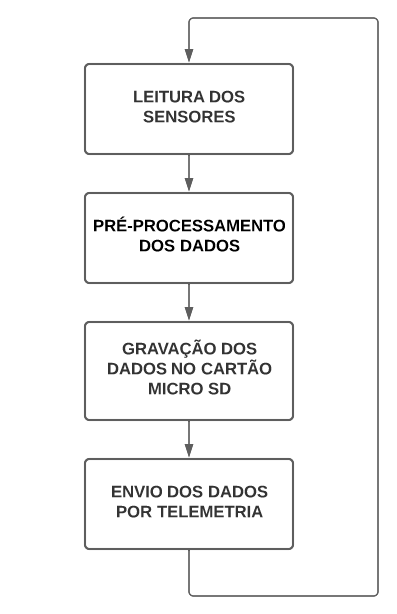
\includegraphics[width=0.50\textwidth]{img/Fluxograma_Firmware1.png}
    \end{center}
    \vspace{-0.5cm}
    \legend{\ABNTEXfontereduzida \textbf{Fonte: O autor.}}
    %\citeonline{BNO055}.}
    \label{fig:Fluxograma_firmware1}
\end{figure}.

\newpage

\subsection{Firmware Receptor}

 Por se tratar de  um sistema cuja finalidade é apenas receber os dados do foguete e enviar os dados para um computador, o firmware do receptor é mais simples do que o firmware do transmissor como é mostrado na figura \ref{fig:Fluxograma_firmware2}.




\begin{figure}[ht]
    \centering
    \caption{Fluxograma firmware do sistema no solo.}
    \begin{center}
        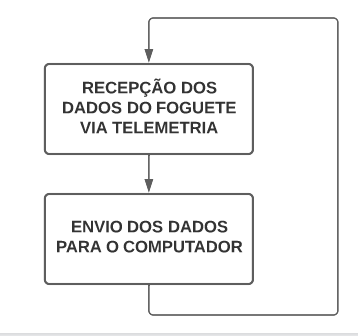
\includegraphics[width=0.45\textwidth]{img/Fluxograma_Firmware2.png}
    \end{center}
    \vspace{-0.5cm}
    \legend{\ABNTEXfontereduzida \textbf{Fonte: O autor.}}
    %\citeonline{BNO055}.}
    \label{fig:Fluxograma_firmware2}
\end{figure}.
 
 
 


\newpage



\section{Viabilidade econômica}

 A viabilidade econômica é um fator importante para este projeto, visto que o recurso financeiro obtido pela equipe tem como origem principal as doações pessoais. Então, todos os componentes foram escolhidos tendo em vista o melhor custo-benefício. O orçamento foi realizado para o sistema embarcado do foguete mostrado na tabela \ref{tab:Orçamento1}, para o sistema em solo mostrado na tabela \ref{tab:Orçamento2} e por fim o valor total do projeto visto na tabela \ref{tab:Orçamento3}.


 


\begin{table}[!thb]
	\centering
	\caption{Preço dos componentes para o sistema embarcado do foguete em 21/03/2022.}
    \begin{adjustbox}{max width={\textwidth},keepaspectratio}%
	\begin{tabular}{|ll|c|c|}
		\cline{3-4}
		\multicolumn{1}{c}{\textbf{}} & 
		\multicolumn{1}{c|}{\textbf{}} & 
		\multicolumn{2}{l|}{\textbf{Preço + Frete}} 
		\\ \cline{1-4}
		 & \multicolumn{1}{c|}{\textbf{Componente}} & \textbf{(USD)} & \textbf{(BRL)}
		 \\ \hline
		& \multicolumn{1}{c|}{STM32F103C8} & 6.92 & 36,47
		 \\ \hline
        & \multicolumn{1}{c|}{V2 Link} & 6.92 & 36,47
		 \\ \hline
        & \multicolumn{1}{c|}{ GPS NEO-6M } & 8.33 & 43,56
		 \\ \hline
        & \multicolumn{1}{c|}{Sensor BNO055} & 39.49 & 208,13
		 \\ \hline
        & \multicolumn{1}{c|}{Sensor BME280} & 9.59 & 50,46
		 \\ \hline
        & \multicolumn{1}{c|}{Radio Lora } & 20.72 & 66,04
		 \\ \hline
        & \multicolumn{1}{c|}{2 Antena radio lora} & 8.00 & 41,53
		 \\ \hline
		 
		 
		 
		 
		 & \multicolumn{1}{c|}{\textbf{Total}} & \textbf{99.97} & \textbf{482,66}
		 \\ \hline

	\end{tabular}
    \end{adjustbox}
%	\Ididthis
	\legend{\ABNTEXfontereduzida \textbf{Fonte:} O autor.}
    \label{tab:Orçamento1} 
\end{table}



Devido a escassez de circuitos eletrônicos e ao aumento do dólar de 4,30 em 11/02/2020 para 5,02  em 2022 causado pela pandemia alguns dos sensores ficaram bastante caros comparado com o valor adquirido no ano de 2020, como é o caso do sensor BNO055 que foi adquirido por 7.22 dólares em 2020 e no ano de 2022 está por 39.49 dólares.  











\begin{table}[!thb]
	\centering
	\caption{Preço dos componentes para o sistema embarcado em solo em 21/03/2022.}
    \begin{adjustbox}{max width={\textwidth},keepaspectratio}%
	\begin{tabular}{|ll|c|c|}
		\cline{3-4}
		\multicolumn{1}{c}{\textbf{}} & 
		\multicolumn{1}{c|}{\textbf{}} & 
		\multicolumn{2}{l|}{\textbf{Preço + Frete}} 
		\\ \cline{1-4}
		 & \multicolumn{1}{c|}{\textbf{Componente}} & \textbf{(USD)} & \textbf{(BRL)}
		 \\ \hline
		& \multicolumn{1}{c|}{STM32F103C8} & 6.92 & 36,47
		 \\ \hline
        & \multicolumn{1}{c|}{Radio Lora } & 20.72 & 66,04
		 \\ \hline

		 
		 
		 
		 
		 & \multicolumn{1}{c|}{\textbf{Total}} & \textbf{27.64} & \textbf{102,51}
		 \\ \hline

	\end{tabular}
    \end{adjustbox}
%	\Ididthis
	\legend{\ABNTEXfontereduzida \textbf{Fonte:} O autor.}
    \label{tab:Orçamento2} 
\end{table}






\begin{table}[!thb]
	\centering
	\caption{Preço total dos sistemas em 21/03/2022.}
    \begin{adjustbox}{max width={\textwidth},keepaspectratio}%
	\begin{tabular}{|ll|c|c|}
		\cline{3-4}
		\multicolumn{1}{c}{\textbf{}} & 
		\multicolumn{1}{c|}{\textbf{}} & 
		\multicolumn{2}{l|}{\textbf{Preço + Frete}} 
		\\ \cline{1-4}
		 & \multicolumn{1}{c|}{\textbf{Componente}} & \textbf{(USD)} & \textbf{(BRL)}
		 \\ \hline
		& \multicolumn{1}{c|}{Sistema embarcado do foguete} & 99.97 & 482,66
		 \\ \hline
        & \multicolumn{1}{c|}{Sistema embarcado em solo } & 27.64 & 102,51
		 \\ \hline

		 
		 
		 
		 
		 & \multicolumn{1}{c|}{\textbf{Total}} & \textbf{127.61} & \textbf{585,17}
		 \\ \hline

	\end{tabular}
    \end{adjustbox}
%	\Ididthis
	\legend{\ABNTEXfontereduzida \textbf{Fonte:} O autor.}
    \label{tab:Orçamento3} 
\end{table}


















\begin{comment}
\begin{table}[!thb]
	%\huge
    \centering
    \caption{Preço dos componentes a serem utilizados 21/03/2022.}
    \begin{adjustbox}{max width={\textwidth},keepaspectratio}%
    \begin{tabular}{@{} p{6.5cm}|c|c|c| }
        \toprule
        \textbf{Componente}
        & Preço incluindo frete (USD) & 
        \\ \hline
        STM32F103C8
        & 6.92   &   36,47   
        \\ \hline
        V2 Link
        & 6.92   &  36,47  
        \\ \hline
        GPS NEO-6M 
        & 8.33   & 43,56
        \\
        \bottomrule
    \end{tabular}
    \end{adjustbox}
    \legend{\ABNTEXfontereduzida \textbf{Fonte:} O autor.}
    \label{tab:cronograma} 
    % \legend{\textbf{Fonte:} O autor.}
\end{table}

\end{comment}






%--------------------------------------------------------------------------------------
% Insere a seção de cronograma
%--------------------------------------------------------------------------------------



\newpage



\section{Cronograma} 
\label{sec:crono}

%A tabela \ref{tab:cronograma} mostra o cronograma de atividades a serem executadas para o TCC II, com base no calendário de 201X.Y da UNIVASF.

A Tabela \ref{tab:cronograma} mostra o cronograma de atividades a serem executadas para o Trabalho de Conclusão II (TCC II), com base no calendário do período 2021.2 da UNIVASF, definido pelo Calendário Acadêmico 2021 da instituição.

\begin{table}[!thb]
	%\huge
    \centering
    \caption{Cronograma das atividades previstas para o TCC II.}
    \begin{adjustbox}{max width={\textwidth},keepaspectratio}%
    \begin{tabular}{@{} p{6.5cm}|c|c|c|c|c|c @{}}
        \toprule
        \textbf{Atividade}
        & Mai & Jun & Jul & Ago & Set & Out
        \\ \hline
        Teste dos sensores individualmente em bancada 
        & X   &     &     &     &     &          
        \\ \hline
        Teste do modulo de Telemetria em bancada
        & X   &     &     &     &     &          
        \\ \hline
        Desenvolvimento da PCB
        &    & X   & X    &     &     &          
        \\ \hline
        Teste completo da PCB em bancada
        &     &    & X   &     &     &          
        \\ \hline
        Teste do sistema em um minifoguete 
        &     &    &    & X    &     &    
        \\ \hline
        Escrita do TCC II                       
        & X   & X   & X   & X   &    &         
        \\ \hline
        Defesa do TCC II                        
        &     &     &     &     & X   &        
        \\
        \bottomrule
    \end{tabular}
    \end{adjustbox}
    \legend{\ABNTEXfontereduzida \textbf{Fonte:} O autor.}
    \label{tab:cronograma} 
    % \legend{\textbf{Fonte:} O autor.}
\end{table}


	%	\chapter{Resultados} \label{ch:RD}



\section{Seção de exemplo 1 - Códigos} \label{sec:resex1}

\subsection{Subseção de exemplo 1 - Inserindo trechos de códigos}
 
O nosso querido Leonardo Cavalcante providenciou um comando que deixa nossos trechos de códigos bonitinhos e gera um elemento pré-textual de Lista de Códigos. 

Os códigos são adicionados através do comando seguinte:

\textbackslash sourcecode\{ Descrição \}\{Label\}\{Linguagem\}\{Arquivo com extensão\}

Um exemplo pode ser visto no código \ref{cmd:cron} abaixo.

\sourcecode{Configuração do intervalo de execução no Script Agendador}{cron}{javascript}{cron.js}


\section{Seção de exemplo 2 - Listas} \label{sec:resex2}

\subsection{Subseção de exemplo 2 - Lista de itens} 

Existem alguns tipos de listas no Latex, iremos exemplificar a lista sem numeração (seção \ref{subsubsec:itemize}), a lista enumerada (seção \ref{subsubsec:enumerate}) e a lista mista (seção \ref{subsubsec:mista}). As listas podem ser encadeadas de diversas maneiras,
de acordo com a necessidade do autor.

\subsubsection{Subsubseção de exemplo 1 - Lista sem numeração} \label{subsubsec:itemize}

Este é um exemplo de lista sem numeração.

\begin{itemize}
	\item \textbf{Cadastrar usuário}

		\begin{itemize}
    		\item Atores
		    	\begin{itemize}
    		    	\item Usuário
		    	\end{itemize}

	    	\item Fluxo de eventos primário
			    \begin{itemize}
	    		    \item o usuário deve se cadastrar informando seu nome, \textit{e-mail} e senha;
		        	\item a API armazena os dados do usuário;
		    	    \item o usuário é liberado para realizar o \textit{login}.
			    \end{itemize}

    		\item Fluxo alternativo
			    \begin{itemize}
		    	   \item o usuário desiste de se cadastrar e cancela o caso de uso clicando no botão voltar.
	    		\end{itemize}

		\end{itemize}
	
\end{itemize}

\subsubsection{Subsubseção de exemplo 2 - Lista enumerada} \label{subsubsec:enumerate}

Este é um exemplo de lista enumerada.

\begin{enumerate}
	\item O Usuário deseja ver o histórico das variáveis climáticas, então através da interface de usuário escolhe o período ao qual o histórico se refere;
	\item A aplicação solicita à API através de uma requisição HTTP contendo o momento de início e o momento do fim do período em seus parâmetros;     			\item A API recebe a solicitação e se comunica com a base de dados, então requere as informações quem possuem a data de leitura no intervalo escolhido;
	\item A base de dados retorna os dados em formato Json para a API;
	\item A API responde à requisição retornando os dados, também em formato Json, para a aplicação cliente;
	\item A aplicação cliente renderiza os gráficos utilizando o conjunto de dados obtidos.
\end{enumerate}

\subsubsection{Subsubseção de exemplo 3 - Lista mista} \label{subsubsec:mista}

Este é um exemplo de lista mista.

\begin{itemize}
	\item \textbf{Cadastrar usuário}

		\begin{itemize}
    		\item Atores
		    	\begin{itemize}
    		    	\item Usuário
		    	\end{itemize}

	    	\item Fluxo de eventos primário
			    \begin{enumerate}
	    		    \item o usuário deve se cadastrar informando seu nome, \textit{e-mail} e senha;
		        	\item a API armazena os dados do usuário;
		    	    \item o usuário é liberado para realizar o \textit{login}.
			    \end{enumerate}

    		\item Fluxo alternativo
			    \begin{itemize}
		    	   \item o usuário desiste de se cadastrar e cancela o caso de uso clicando no botão voltar.
	    		\end{itemize}

		\end{itemize}

	\item \textbf{Visualizar dados atuais}

		\begin{itemize}
		    \item Atores
	    		\begin{itemize}
		    	    \item Usuário
			    \end{itemize}
    
	    	\item Pré-condições
			    \begin{itemize}
		     	   \item o usuário deve estar autenticado
			    \end{itemize}

	    	\item Fluxo de eventos primário
			    \begin{enumerate}
		    	    \item o usuário deve efetuar o \textit{login} informando o \textit{e-mail} e a senha;
	    		    \item caso o usuário não seja autenticado, o sistema informa a respeito de credenciais inválidas e encerra o caso de uso;
		    	    \item a API autentica o usuário;
    			    \item o usuário é liberado para visualizar os dados atuais dos sensores da estação;
		        	\item após a visualização o usuário pode finalizar o caso de uso ou efetuar uma nova consulta se desejar.
			    \end{enumerate}

    		\item Fluxo alternativo
			    \begin{itemize}
    			   \item o usuário desiste de visualizar os dados atuais e cancela o caso de uso clicando no botão voltar.
			    \end{itemize}

		\end{itemize}

	\item \textbf{Visualizar histórico}

		\begin{itemize}
		    \item Atores
	    		\begin{itemize}
		    	    \item Usuário
	    		\end{itemize}

	    	\item Pré-condições
    			\begin{itemize}
			        \item o usuário deve estar autenticado
			    \end{itemize}

		    \item Fluxo de eventos primário
			    \begin{enumerate}
			        \item o usuário deve efetuar o \textit{login} informando o \textit{e-mail} e a senha;
			        \item caso o usuário não seja autenticado, o sistema informa a respeito de credenciais inválidas e encerra o caso de uso;
			        \item a API autentica o usuário;
			        \item o usuário é liberado para escolher qual período cujo histórico será exibido;
			        \item o usuário seleciona as variáveis a serem exibidas no gráficos de linhas;
			        \item após a visualização do histórico o usuário pode finalizar o caso de uso se desejar.
			    \end{enumerate}

		    \item Fluxo alternativo
			    \begin{enumerate}
			        \item após a escolha do período de exibição do histórico o usuário pode voltar para a tela anterior e escolher um novo período;
			        \item o histórico é exibido para o usuário;
			        \item após a visualização do histórico o usuário pode finalizar o caso de uso ou efetuar uma nova consulta se desejar.
			    \end{enumerate}

		    \item Fluxo alternativo
			    \begin{enumerate}
			        \item o usuário desiste de visualizar o histórico e cancela o caso de uso clicando no botão voltar.
			    \end{enumerate}
		\end{itemize}
\end{itemize}
	%	%--------------------------------------------------------------------------------------
% Este arquivo contém a sua conclusão
%--------------------------------------------------------------------------------------
\chapter{Considerações Finais e Trabalhos Futuros}

\lipsum[1-2]
 
\section{Trabalhos futuros}

futuramente poderia trocar o sensor BMP280 por o sensor BME280 para medir temperatura, pressão e humidade

\lipsum[55]

	\postextual
		\bibliography{tex/references}
	%	\begin{anexosenv}
\chapter{Comandos seriais da estação meteorológica \textit{Vantage Vue™}} \label{anex:anexo1}

\begin{center}
\scalefont{0.85}
\begin{longtable}{ll}
\caption{Comandos seriais suportados pela estação meteorológica \textit{Vantage Vue™}}\\
\hline
\multicolumn{1}{c}{\textbf{Instrução}} & \multicolumn{1}{c}{\textbf{Descrição}} \\ \hline
\endfirsthead

\multicolumn{2}{c}%
{{\bfseries \tablename\ \thetable{} -- Continuação da página anterior}} \\

\hline
\multicolumn{1}{c}{\textbf{Instrução}} & \multicolumn{1}{c}{\textbf{Descrição}} \\ \hline
\endhead

\multicolumn{2}{r}{{Continua na próxima página}} \\
\endfoot

\endlastfoot

\multicolumn{2}{c}{\cellcolor{gray!25}\textbf{Comandos de teste}}                                                   		 \\ \hline
\textbf{TESTE}                            & Envia a \textit{string} "TEST\textbackslash n" de volta  \\ \hline
\textbf{WRD}                        & Responde com o tipo de estação meteorológica \\ \hline
\textbf{RXCHECK}                        & Responde com o diagnóstico do Console \\ \hline
\textbf{RXTEST}                       & Muda a tela do console de \textit{"Receiving from"} para tela de dados atuais                                                        \\ \hline
\textbf{VER}                           & Responde com a data do \textit{firmware}                                                             \\ \hline
\textbf{RECEIVERS}                    & Responde com a lista das estações que o console "enxerga" \\ \hline
\textbf{NVER}                       & Responde com a versão do \textit{firmware}                                                             \\ \hline
\multicolumn{2}{c}{\cellcolor{gray!25}\textbf{Comandos de dados atuais}}                                             \\ \hline
\textbf{LOOP}                     & Responde com a quantidade de pacotes especificada a cada 2s        \\ \hline
\textbf{LPS}                & Responde a cada 2s com a quantidade de pacotes diferentes especificada          \\ \hline
\textbf{HILOWS}                & Responde com todo os dados de \textit{high/low}                 \\ \hline
\textbf{PUTRAIN}                      & Seta a quantidade anual de precipitação \\ \hline
\textbf{PUTET}                 & Seta a quantidade anual de evapotranspiração        \\ \hline
\multicolumn{2}{c}{\cellcolor{gray!25}\textbf{Comandos de \textit{download}}}                                     		 \\ \hline
\textbf{DMP}                 & Faz o \textit{download} de todo o arquivo de memória \\ \hline
\textbf{DMAFT}                   & Faz o \textit{download} de todo o arquivo de memória após a data especificada \\ \hline
\multicolumn{2}{c}{\cellcolor{gray!25}\textbf{Comandos da EEPROM}}                                     		 \\ \hline
\textbf{GETEE}                 & Lê toda a memória EEPROM \\ \hline
\textbf{EEWR}                   & Escreve um \textit{byte} de dados à partir do endereço especificado                                   \\ \hline
\textbf{EERD}                   & Lê a quantidade de dados especificada iniciando no endereço especificado                                   \\ \hline
\textbf{EEBWR}                   & Escreve os dados na EEPROM                                    \\ \hline
\textbf{EEBRD}                   & Lê os dados da EEPROM \\ \hline
\multicolumn{2}{c}{\cellcolor{gray!25}\textbf{Comandos de calibração}}                                     		 \\ \hline
\textbf{CALED}                 & Envia os dados da temperatura e umidade corrente para atribuir à calibração \\ \hline
\textbf{CALFIX}                   & Atualiza o \textit{display} quando os números de calibração mudam\\ \hline
\textbf{BAR}                   & Seta os valores da elevação e o \textit{offset} do barômetro quando a localização é alterada                                   \\ \hline
\textbf{BARDATA}                   & Mostra os valores atuais da calibração do barômetro                                   \\ \hline \\
\multicolumn{2}{c}{\cellcolor{gray!25}\textbf{Comandos de limpeza}}                                     		 \\ \hline
\textbf{CLRLOG}                 & Limpa todo o arquivo de dados                                                       \\ \hline
\textbf{CLRALM}                   & Limpa todos os limiares dos alarmes                                   \\ \hline
\textbf{CLRCAL}                   & Limpa todos os \textit{offsets} da calibração da temperatura e da umidade \\ \hline
\textbf{CLRGRA}                   & Limpa o gráfico do console \\ \hline
\textbf{CLRVAR}                   & Limpa o valor da precipitação ou da evapotranspiração \\ \hline
\textbf{CLRHIGHS}                   & Limpa todos os valores de pico diários, mensais ou anuais                                   \\ \hline
\textbf{CLRLOWS}                   & Limpa todos os valores de mínimos diários, mensais ou anuais \\ \hline
\textbf{CLRBITS}                   & Limpa os \textit{bits} de alarme ativos                                  \\ \hline
\textbf{CLRDATA}                   & Limpa todos os dados atuais                                   \\ \hline
\multicolumn{2}{c}{\cellcolor{gray!25}\textbf{Comandos de configuração}}                                     		 \\ \hline
\textbf{BAUD}                 & Atribui o valor do \textit{baudrate} do console                                                       \\ \hline
\textbf{SETTIME}                   & Define a data e a hora do console                                   \\ \hline
\textbf{GAIN}                   & Define o ganho do receptor de rádio                                   \\ \hline
\textbf{GETTIME}                   & Retorna a hora e a data atual do console                                   \\ \hline
\textbf{SETPER}                   & Define o intervalo de arquivamento                                   \\ \hline
\textbf{STOP}                   & Desabilita a criação dos registros                                   \\ \hline
\textbf{START}                   & Habilita a criação dos arquivos \\ \hline
\textbf{NEWSETUP}                   & Reinicia o console após alguma configuração nova                                  \\ \hline
\textbf{LAMPS}                   & Liga ou desliga as lâmpadas do console \\ \hline

%\label{tab:6}
\end{longtable}
\fonte{\citeonline{VSPDOC} (Traduzido).}
\end{center}


\end{anexosenv}


\end{document}
